
%%%%%%%%%%%%%%%%%%%%%%%%%%%%%%%%%%%%%%%%%%%%%%%%%%%%%%%%%%%%%%%%%%%%%%%
%% Haupteil des Dokuments -Main-                                     %%
%%%%%%%%%%%%%%%%%%%%%%%%%%%%%%%%%%%%%%%%%%%%%%%%%%%%%%%%%%%%%%%%%%%%%%%


%% Basierend auf einer TeXnicCenter-Vorlage von Mark M�ller
%%%%%%%%%%%%%%%%%%%%%%%%%%%%%%%%%%%%%%%%%%%%%%%%%%%%%%%%%%%%%%%%%%%%%%%

% W�hlen Sie die Optionen aus, indem Sie % vor der Option entfernen  
% Dokumentation des KOMA-Script-Packets: scrguide

%%%%%%%%%%%%%%%%%%%%%%%%%%%%%%%%%%%%%%%%%%%%%%%%%%%%%%%%%%%%%%%%%%%%%%%
%% Optionen zum Layout des Buchs                                     %%
%%%%%%%%%%%%%%%%%%%%%%%%%%%%%%%%%%%%%%%%%%%%%%%%%%%%%%%%%%%%%%%%%%%%%%%
\documentclass[
%a5paper,							% alle weiteren Papierformat einstellbar
%landscape,						% Querformat
12pt,								% Schriftgr��e (12pt, 11pt (Standard))
%BCOR 1cm,							% Bindekorrektur, bspw. 1 cm
%DIVcalc,							% f�hrt die Satzspiegelberechnung neu aus
twoside ,							% s. scrguide 2.4
%oneside,							% einseitiges Layout
%twocolumn,						% zweispaltiger Satz
%openany,							% Kapitel k�nnen auch auf linken Seiten beginnen
openright,
%openleft,
%halfparskip*,				% Absatzformatierung s. scrguide 3.1
%headsepline,					% Trennline zum Seitenkopf	
%footsepline,					% Trennline zum Seitenfu�
%notitlepage,					% in-page-Titel, keine eigene Titelseite
%chapterprefix,				% vor Kapitel�berschrift wird "Kapitel Nummer" gesetzt
%appendixprefix,				% Anhang wird "Anhang" vor die �berschrift gesetzt 
%normalheadings,			% �berschriften etwas kleiner (smallheadings)
%idxtotoc,						% Index im Inhaltsverzeichnis
%liststotoc,					% Abb.- und Tab.verzeichnis im Inhalt
%bibtotoc,						% Literaturverzeichnis im Inhalt
%leqno,								% Nummerierung von Gleichungen links
%fleqn,								% Ausgabe von Gleichungen linksb�ndig
%draft								% �berlangen Zeilen in Ausgabe gekennzeichnet
]
{scrbook}

\usepackage{chngcntr}
\counterwithout{equation}{chapter}
%\pagestyle{empty}		% keine Kopf und Fu�zeile (k. Seitenzahl)
%\pagestyle{headings}	% lebender Kolumnentitel  

%% Deutsche Anpassungen %%%%%%%%%%%%%%%%%%%%%%%%%%%%%%%%%%%%%
\usepackage[english]{babel}
%\usepackage[ngerman]{babel}
\usepackage[utf8]{inputenc}
%\usepackage[ansinew]{inputenc}
%\usepackage[latin1]{inputenc}
%\usepackage[T1]{fontenc}
%\usepackage[scaled]{helvet}
\usepackage{arydshln}  %for dashlines
%lines for tabes



%% Falls die automatische Worttrennung in W�rtern mit Umlauten
%% nicht funktionieren sollte oder der Text pixelig aussieht:
%% ==> Installieren Sie die cm-super Fonts (z.B. mit dem mikTeX Package Manager).
%% Eine nicht ganz vollwertige Alternative ist die Verwendung dieses Pakets:
\usepackage{ae, aeguill}


%% Packages f�r Grafiken & Abbildungen %%%%%%%%%%%%%%%%%%%%%%
\usepackage{graphicx} %%Zum Laden von Grafiken
%\usepackage{subfig} %%Teilabbildungen in einer Abbildung
%\usepackage{pst-all} %%PSTricks - nicht verwendbar mit pdfLaTeX

\usepackage{float} % f�r eine bessere Positionierung von Grafiken

\usepackage{wrapfig}

\usepackage{listliketab}  %f�r die getabbte itemize



\usepackage[usenames]{color}
\definecolor{rot}{RGB}{255,195,195}
\definecolor{dunkelblau}{RGB}{160,172,254}
\definecolor{hellblau}{RGB}{164,215,216}
\definecolor{gelb}{RGB}{254,247,205}
\definecolor{gruen}{RGB}{218,255,204}
\definecolor{lila}{RGB}{205,181,217}
\definecolor{Gray}{gray}{0.5}

\usepackage{colortbl}    %um Tabellen farbig zu machen
\usepackage[table]{xcolor}% http://ctan.org/pkg/xcolor

%% Beachten Sie:
%% Die Einbindung einer Grafik erfolgt mit \includegraphics{Dateiname}
%% bzw. �ber den Dialog im Einf�gen-Men�.
%% 
%% Im Modus "LaTeX => PDF" k�nnen Sie u.a. folgende Grafikformate verwenden:
%%   .jpg  .png  .pdf  .mps
%% 
%% In den Modi "LaTeX => DVI", "LaTeX => PS" und "LaTeX => PS => PDF"
%% k�nnen Sie u.a. folgende Grafikformate verwenden:
%%   .eps  .ps  .bmp  .pict  .pntg


%% Bibliographiestil %%%%%%%%%%%%%%%%%%%%%%%%%%%%%%%%%%%%%%%%%%%%%%%%%%
%\usepackage{natbib}



%%  (Franz Gritschneder hinzugef�gte Bibliotheken)

\usepackage{setspace}

\usepackage{fancyhdr}							%f�r Kopf- und Fusszeilen



\usepackage{lettrine}   % f�r Initialen an einem Abschnitt z.B. \lettrine[lines=1]{H}{}auptaug 

%\usepackage[a4paper,
%left=3cm, right=3cm,
%top=3cm,
% bottom=2cm]{geometry}

\usepackage{pgfplots} %diagrams
\usepackage{yfonts}   %Initialen

%\usepackage[T1]{fontenc} % �ndert die Fontkodierung auf T1 Format
\usepackage{pdfpages}
%\ pdf einbinden

%\parindent0mm  % Absatzeinrückung stoppen

%graphics
%\usepackage[demo]{graphicx}
\usepackage{subfig}
\usepackage{tabularx} %fancy tables
%\usepackage{arydshln} %for hdashlines in tables

\usepackage{listings} %for pseudo code

\lstset{
		frame=tb
	}

\usepackage[linesnumbered,ruled]{algorithm2e} %for pseudo code
\DontPrintSemicolon 

%\usepackage[ps2pdf,%
%linktocpage,%
%colorlinks,%
%bookmarks,%
%bookmarksopen,%
%bookmarksnumbered]{hyperref}


\usepackage{multirow}    % f�r die Tabellenumgebung
%\usepackage{multicolumn} % f�r die Tabellenumgebung - 


\setcounter{secnumdepth}{3}  %gibt die Tiefe der Nummerierung f�r Unterpunkte an

%\chapter{Kapitel1}
%\section{Punkt1}
%\subsection{Unterpunkt1}
%\subsubsection{Unterpunkt2}
%\paragraph{Unterpunkt3}
%\subparagraph{Unterpunkt4


\newcommand{\entspr}{\ensuremath \widehat{=}}


%\setlength{\parindent}{0pt} %kein Einzug auf der 1. Zeile eines Absatzes


\usepackage{textcomp}
 %Mathematikbefehle anzeigen
%\usepackage{mathtools} 
 \usepackage{amsmath}
 \usepackage{amssymb}
 
 \newcommand*{\nobarfrac}[2]{\genfrac{  \langle}{ \rangle}{0pt} {} {#1}{#2}}
 
 %Zur Erzeugung von Index
 \usepackage{makeidx}
 %Index erstellen
 \makeindex
 
  %captionbefehle 
 \usepackage{caption} 
 \captionsetup{labelfont=bf, font={small,sf}}
 

 \usepackage{hyperref}
 
 
% \usepackage[colorlinks=true,        %zur anzeige der bookmarks im pdf-ausgabefile
%        linkcolor=black,
%        citecolor=black,
%%        linkcolor=blue,
%%        citecolor=red,
%        filecolor=black,
%        %pagecolor=black,
%        urlcolor=black,
%        bookmarks=true,
%        bookmarksopen=false,
%        bookmarksopenlevel=5,
%        bookmarksnumbered,
%        plainpages=false,
%        pdfpagelabels=true]{hyperref}
%\hypersetup{%
%pdftitle = {Text},
%pdfsubject = {Text},
%pdfauthor = {Text},
%pdfkeywords = {Text},
%pdfcreator = {GNU Ghostscript 8.00},
%pdfproducer = {LaTeX},
%urlcolor = blue
%}

 

 
 

\makeatletter
\renewenvironment{thebibliography}[1]
{\chapter{Bibliography}%
%{\chapter{\refname}%
\@mkboth{\MakeUppercase\refname}{\MakeUppercase\refname}%
\list{\@biblabel{\@arabic\c@enumiv}}%
{\settowidth\labelwidth{\@biblabel{#1}}%
\leftmargin\labelwidth
\advance\leftmargin\labelsep
\@openbib@code
\usecounter{enumiv}%
\let\p@enumiv\@empty
\renewcommand\theenumiv{\@arabic\c@enumiv}}%
\sloppy
\clubpenalty4000
\@clubpenalty \clubpenalty
\widowpenalty4000%
\sfcode`\.\@m}
{\def\@noitemerr
{\@latex@warning{Empty `thebibliography' environment}}%
\endlist}
\makeatother


\renewcommand{\headrulewidth}{0.0pt}    %Dicke der Kopflinie
\renewcommand{\footrulewidth}{0.0pt}    %Dicke der Fusslinie

\setlength{\textheight}{630pt}%630
\setlength{\textwidth}{450pt}
%\setlength{\textwidth}{17cm}
\setlength{\headsep}{40pt}
\setlength{\headheight}{50pt}%45


%***** page style settings *****
%For the beginning we dont display chapters, only pages

\pagestyle{fancy}
\fancyhf{}
%\fancyhead[LE,RO]{\leftmark}   %current chapter and section on the outer side header
%\fancyhead[RE,LO]{\thechapter}
%\fancyfoot[CE,CO]{\rightmark}  %next chapter and section in the center bot
\fancyfoot[LE,RO]{\thepage}  %page number on the outer bottom side

%\renewcommand{\headrulewidth}{2pt}  %thickness of the top line
%\renewcommand{\footrulewidth}{1pt}  %thickness of the bottom line







\begin{document}


%%%%%%%%%%%%%%%%%%%%%%%%%%%%%%%%%%%%%%%%%%%%%%%%%%%%%%%%%%%%%%%%%%%%%%%
%% Ihr Buch                                                          %%
%%%%%%%%%%%%%%%%%%%%%%%%%%%%%%%%%%%%%%%%%%%%%%%%%%%%%%%%%%%%%%%%%%%%%%%
%% Schmutztitel-Seite %%%%%%%%%%%%%%%%%%%%%%%%%%%%%%%%%%%%%%%%%%%%%%%%%
%\extratitle{Schmutztitel}

%% eigene Titelseitengestaltung %%%%%%%%%%%%%%%%%%%%%%%%%%%%%%%%%%%%%%%    
%\begin{titlepage}
%Einsetzen der TXC Vorlage "Deckblatt" m?glich
%\end{titlepage}

%\include{chapters/Deckblatt}

%% Angaben zur Standardformatierung des Titels %%%%%%%%%%%%%%%%%%%%%%%%
%\titlehead{Titelkopf}
%\subject{Typisierung}
%%%%%%%%%%%%%%%%%%%%%%%%%%%%%%%%%%%%%%%%%%%%%%%%%%\title{Der Name Ihrer Arbeit}
%%%%%%%%%%%%%%%%%%%%%%%%%%%%%%%%%%%%%%%%%%%%%%%%%%%%%%%\author{Ihr Name}
%\and{Der Name des Co-Autoren}
%\thanks{Fu?note}			% entspr. \footnote im Flie?text
%\date{}							% falls anderes, als das aktuelle gew?nscht
%\publishers{Herausgeber}

%% R?ckseite der Titelseite %%%%%%%%%%%%%%%%%%%%%%%%%%%%%%%%%%%%%%%%%%%
%\uppertitleback{Titelr?ckseitenkopf}
%\lowertitleback{Titelr?ckseitenfu?}

%% Widmungsseite %%%%%%%%%%%%%%%%%%%%%%%%%%%%%%%%%%%%%%%%%%%%%%%%%%%%%%
%\dedication{Widmung}

%\maketitle 						% Titelei wird erzeugt

%% %%%%%%%%%%%%%%%%%%%%%%%%%%%%%%%%%%%%%%%%%%%%%%%%%%%%%%%%%%%%%%%%%%%5

\begingroup %group removes the 1.paeg of chapter on right side -> empty pages
\renewcommand{\cleardoublepage}{}
\renewcommand{\clearpage}{}

\frontmatter   %einleitungsteil   % Vorspann (z.B. roemische Seitenzahlen)





\begin{titlepage}

\begin{center}
	\LARGE Eberhard Karls Universität Tübingen\\
	\large Mathematisch-Naturwissenschaftliche Fakultät \\
	Wilhelm-Schickard-Institut für Informatik\\
	[3cm]
	\huge Bachelorarbeit Kognitionswissenschaft\\
	[2cm]
	\Large\textbf{Inverse Classification using Generative Models}\\
	[1.5cm]
	\large Marius Hobbhahn\\
	[0.5cm]
	Eingereicht am: \\
	17.10.2018\\
	\vfill
	\small\textbf{Gutachter}\\[0.3cm]
	\large Prof. Martin Butz\\
	\footnotesize Wilhelm-Schickard-Institut für Informatik\\Universität Tübingen\\
	[1cm]
	\small\textbf{Betreuer}\\[0.3cm]
	\large Dr. Sebastian Otte\\
	\footnotesize Wilhelm-Schickard-Institut für Informatik\\Universität Tübingen\\
\end{center}
\newpage
\thispagestyle{empty}
\vspace*{\fill}
\noindent
\textbf{Hobbhahn, Marius:}\\
\emph{Inverse classification using generative models}\\
Bachelorarbeit Kognitionswissenschaft\\
Eberhard Karls Universität Tübingen\\
Bearbeitungszeitraum: 18.06.18 - 18.10.18
%\includepdf[fitpaper]{images/cover.pdf}


\end{titlepage}
	

\onehalfspacing % zeilen abstand 1.5

\thispagestyle{empty}

\begingroup

\noindent
\textbf{\LARGE Abstract}\\
\parskip 12pt \\
Training a forward model and using temporal gradients has been successfully deployed in the domain of motion control. Inverse classification is a new technique in which a generative model is used both as a generator and a classifier. The generative model is first used to produce sequences given one-hot vectors representing classes as input. In the second step the network is fed a uniformly distributed vector that is iteratively adapted with the gradients resulting from the loss between the generated sequence and a target sequence. In the optimal case, the input converges towards the one-hot vector representing the class of the target sequence. To test the performance of inverse classification multiple experiments were conducted on sequences representing handwritten characters. \\
The technique of inverse classification is able to compete with a standard classification approach for less complex tasks but performs significantly worse on data of higher complexity.
\endgroup

\pagebreak

\begingroup

\noindent
\textbf{\LARGE Zusammenfassung}\\
\parskip 12pt \\
Das Training eines Vorwärtsmodells und die anschließende Nutzung von Gradienten wurde bereits erfolgreich im Bereich der Bewegungssteuerung eingesetzt. Inverse Klassifizierung ist eine neuartige Technik, die ein generatives Modell sowohl als Generator als auch zur Klassifizierung nutzt. Das Vorwärtsmodell wird erst darauf trainiert Sequenzen, die Klassen repräsentieren, zu generieren. Im Klassifizierungsschritt wird dem Netzwerk zunächst ein gleichverteilter Vektor gefüttert, welcher iterativ mit den Gradienten angepasst wird. Der Gradient entsteht aus dem Fehler zwischen dem Ergebnis des Vorwärtsprozesses und dem zu klassifizierenden Ziel. Im Optimalfall konvergiert der Eingangsvektor gegen den one-hot Vektor, der die Klasse der Zielsequenz repräsentiert. Um die Leistung der neuen Technik zu testen, wurden verschiedene Experimente auf einem Datensatz von Sequenzen, die handgeschriebenen Buchstaben entsprechen, ausgeführt.\\
Die Technik der Inversen Klassifizierung liefert bei weniger komplexen Aufgaben Resultate, die vergleichbar zu einer Standard Klassifizierung sind, aber schneidet bei höherer Komplexität merkbar schlechter ab. 
\vspace*{\fill}

\endgroup
\newpage
\tableofcontents






\singlespacing %zeilenabstand 1.0
%% Erzeugung von Verzeichnissen %%%%%%%%%%%%%%%%%%%%%%%%%%%%%%%%%%%%%%%
\setcounter{page}{1} % seitenzahl ab inhatsverzeichniss
\addtocontents{toc}{\protect\thispagestyle{fancy}} 
%\tableofcontents			% Inhaltsverzeichnis
%\newpage
%\addtocontents{lof}{\protect\thispagestyle{fancy}}  
%\listoffigures				% Abbildungsverzeichnis
%\newpage
%\addtocontents{lot}{\protect\thispagestyle{fancy}} 
%\listoftables				% Tabellenverzeichnis

\endgroup



%% Der Text %%%%%%%%%%%%%%%%%%%%%%%%%%%%%%%%%%%%%%%%%%%%%%%%%%%%%%%%%%%
\onehalfspacing
%\doublespacing


%\cleardoublepage
%$$$$$$$$$$$$$$$$$$$$$$$$$$$$$$$$$$$$$$$$$$$$$$$$$$



\mainmatter
\newcounter{romcounter}
\setcounter{romcounter}{\value{page}}
\renewcommand{\thepage}{\arabic{page}}
\renewcommand{\chapterpagestyle}{empty} % first page of chapter now heading
\setcounter{page}{1}

\onehalfspacing

%***** page style settings *****
\pagestyle{fancy}
\fancyhf{}
\fancyhead[LE,RO]{\leftmark}   %current chapter and section on the outer side header
%\fancyhead[RE,LO]{\thechapter}
\fancyfoot[CE,CO]{\rightmark}  %next chapter and section in the center bot
\fancyfoot[LE,RO]{\thepage}  %page number on the outer bottom side

\renewcommand{\headrulewidth}{2pt}  %thickness of the top line
\renewcommand{\footrulewidth}{1pt}  %thickness of the bottom line

%$$$$$$$$$$$$$$$$$$$$$$$$$$$$$$$$$$$$$$$$$$$$$$$$$$$$
% Main chapter 1:
% Introduction 

\chapter{Introduction}
\label{chap:Introduction}

Learning a forward model and then using temporal gradients has been shown to generate active-inference-based, flexible, adaptive goal-directed behavior in the domain of planning future trajectories in partially observable environments \cite{RocketballOtte2017}. The model has been successfully extended to not only include the prospective inference but also a retrospective inference process, i.e. inferring the unobservable contextual state that best explains its recently encountered sensorimotor experiences \cite{REPRISE2018}. In both cases, the gradient based inference was not only highly successful but even able to be used in online applications for very fast moving vehicles in partially observable environments. \\
Autoencoders are a class of artificial neural networks, combining an encoder and a decoder network. The encoder is used to reduce the dimensionality of the input data to a minimum while still maintaining all necessary features. The space of all possible options after the dimensionality reduction is called latent space. The decoder reconstructs the original input from the reduced dimensionality of the latent space. The autoencoder therefore extracts the essential features from the input to then generate the inputs again from these essential features. Many different versions of autoencoders have been published since their first appearance, including but not limited to: Variational Autoencoders \cite{2013VAE} and Denoising Autoencoders \cite{DenoisingAutoencodersVincent2010}. \\
Generative models have been able to create sequences that are indistinguishable to sequences created by humans. In the field of handwritten characters, Nikolaus (\cite{2018Nikolaus}) was able to show that a recurrent neural network (RNN) with the usage of long short-term memory (LSTM) is able to generate characters and variations of characters, by combining different versions of learned data. \\
This work is extracting and combining ideas from the previously described concepts. It attempts to implement a generative model to create handwritten characters and use the temporal gradients to then infer the original inputs when given certain outputs. Essentially it is like an autoencoder in the same model, where the main processes swapped positions. The forward process is the decoder part while the inverse classification can be thought of an encoder. \\
If the technique can be successfully deployed multiple advantages can be gained. First, there would be one model that can generate and classify at the same time. This means that only half the training time is necessary in comparison to training a generator and a classifier individually. Second, significantly less training data could be used. If the model is able to generate the sequences, it very likely learned a concept about the essential features of that sequence and its differentiation to other concepts. This includes different variations of this sequence and therefore makes massive amounts of training data unnecessary. This would speed up the training process and make classification problems, for which only few data exist, possible to be classified. 

 
% Main chapter 2:
\chapter{Theory}
\label{chap:theory}

\section{Recurrent Neural Networks}

Recurrent neural networks (RNNs) are optimal for processing sequential information. Some data are structured in a way in which the order of presentation is very important or parts of the problem can only be understood when having already seen previous information. Take the following sentence as an example: ``The dog barked at the cat'' has an entirely different meaning than ``The cat barked at the dog''. Another example would be weather data. If it rained the first 3 days and then got sunny for the rest of the week my prediction would be very different than if it was sunny the first 3 days and then started to rain. The RNN is able to process exactly that sequential component of the data. It extends a multilayer perceptron 
\cite{Rosenblatt58theperceptron:} by having recurrent connections within the hidden layers. This means that for every entry but the first in the sequence every neuron not only gets information from the new input but also from its previous timestep. A graphical demonstration can be found in figure \ref{fig:RNN}.

\begin{figure}[!htb]
	\centering
	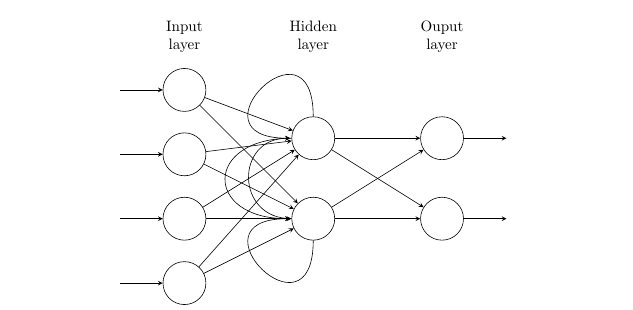
\includegraphics[width=0.7\textwidth]{images/RNN.png}
	\caption{Depiction of a recurrent neural network. Figure taken from \protect\footnotemark}
	\label{fig:RNN}
\end{figure}

The network can be unfolded over time to make the concepts easier to understand. For this the dimension is explicitly added. On the x-axis of figure \ref{fig:unfolded_RNN} 

\begin{figure}[!htb]
	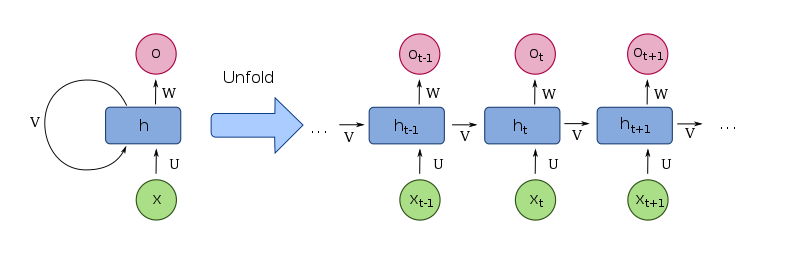
\includegraphics[width=0.9\textwidth]{images/unfolded_RNN.png}
	\caption{Depiction of a recurrent neural network unfolded over time. Figure taken from \protect\footnotemark}
	\label{fig:unfolded_RNN}
\end{figure}


\footnotetext{\url{https://tex.stackexchange.com/questions/364413/drawing-an-unfolded-recurrent-neural-network}}
\footnotetext{\url{https://en.wikipedia.org/wiki/File:Recurrent_neural_network_unfold.svg}}

the inputs are plotted in increasing chronological order. Now it is very clearly visible that the output of every cell is determined not only by its input at timestep $t$ but also from its own state at timestep $t-1$. \\
To train the network, backpropagation is modified to become backpropagation through time \cite{werbos_backpropagation_1990}, i.e. the gradient of the error is backpropagated through the network and the weights of the connections are adapted accordingly. 

\section{Vanishing Gradient Problem}

A problem with gradient-based learning is that the adaptions of the weights in early layers become vanishingly small when the number of layers becomes larger. This is due to the fact that the network weights are updated by the chain rule, i.e. they are updated proportional to the partial derivative of the error function with respect to the current weight. An example of the chainrule for the adaption of the weights to the output layer is given in equations \ref{eq:chain_rule_first} to \ref{eq:chain_rule_last}. $E, w_{ij}, o_j, v_j, \varphi$ are the error, weight, output of a neuron, weighted sum of inputs and activation function respectively.\\
When many layers are involved, the updates become exponentially smaller with an increasing number of layers between weight and output layer since the chain of derivatives gets increasingly longer. Given that for many sequential problems long sequences are used, backpropagation through time would either take incredibly long to train or not adapt weights for very early entries. To solve this problem long short-term memories were developed.


\begin{align}
	\frac{\partial E}{\partial w_{ij}} &= \frac{\partial E}{\partial o_j} \cdot \frac{\partial o_j}{\partial v_j} \cdot \frac{\partial v_j}{w_{ij}}
	\label{eq:chain_rule_first} \\
	\frac{\partial v_j}{\partial w_{ij}} &= \frac{\partial}{\partial w_{ij}}(\sum_{k = 1}^{n} w_{kj}o_k) = \frac{\partial}{\partial w_{ij}} w_{ij} o_i = o_i\\
	\frac{\partial o_j}{\partial v_j} &= \varphi'(v_j)
	\label{eq:chain_rule_last}
\end{align}




\section{Long Short-Term Memory (LSTM)}
\label{section:LSTM}

Long short-term memories (LSTMs) were developled in 1997 by Hochreiter and Schmidhuber \cite{LSTMHochreiter1997} to solve the vanishing gradient problem. An LSTM unit is composed of a cell with input gate, output gate and forget gate. The cell saves information over time like a buffer and the gates are used to control the flow of information in and out of the cell. A visualization can be seen in figure \ref{fig:LSTM}.

\begin{figure}[!htb]
	\centering
	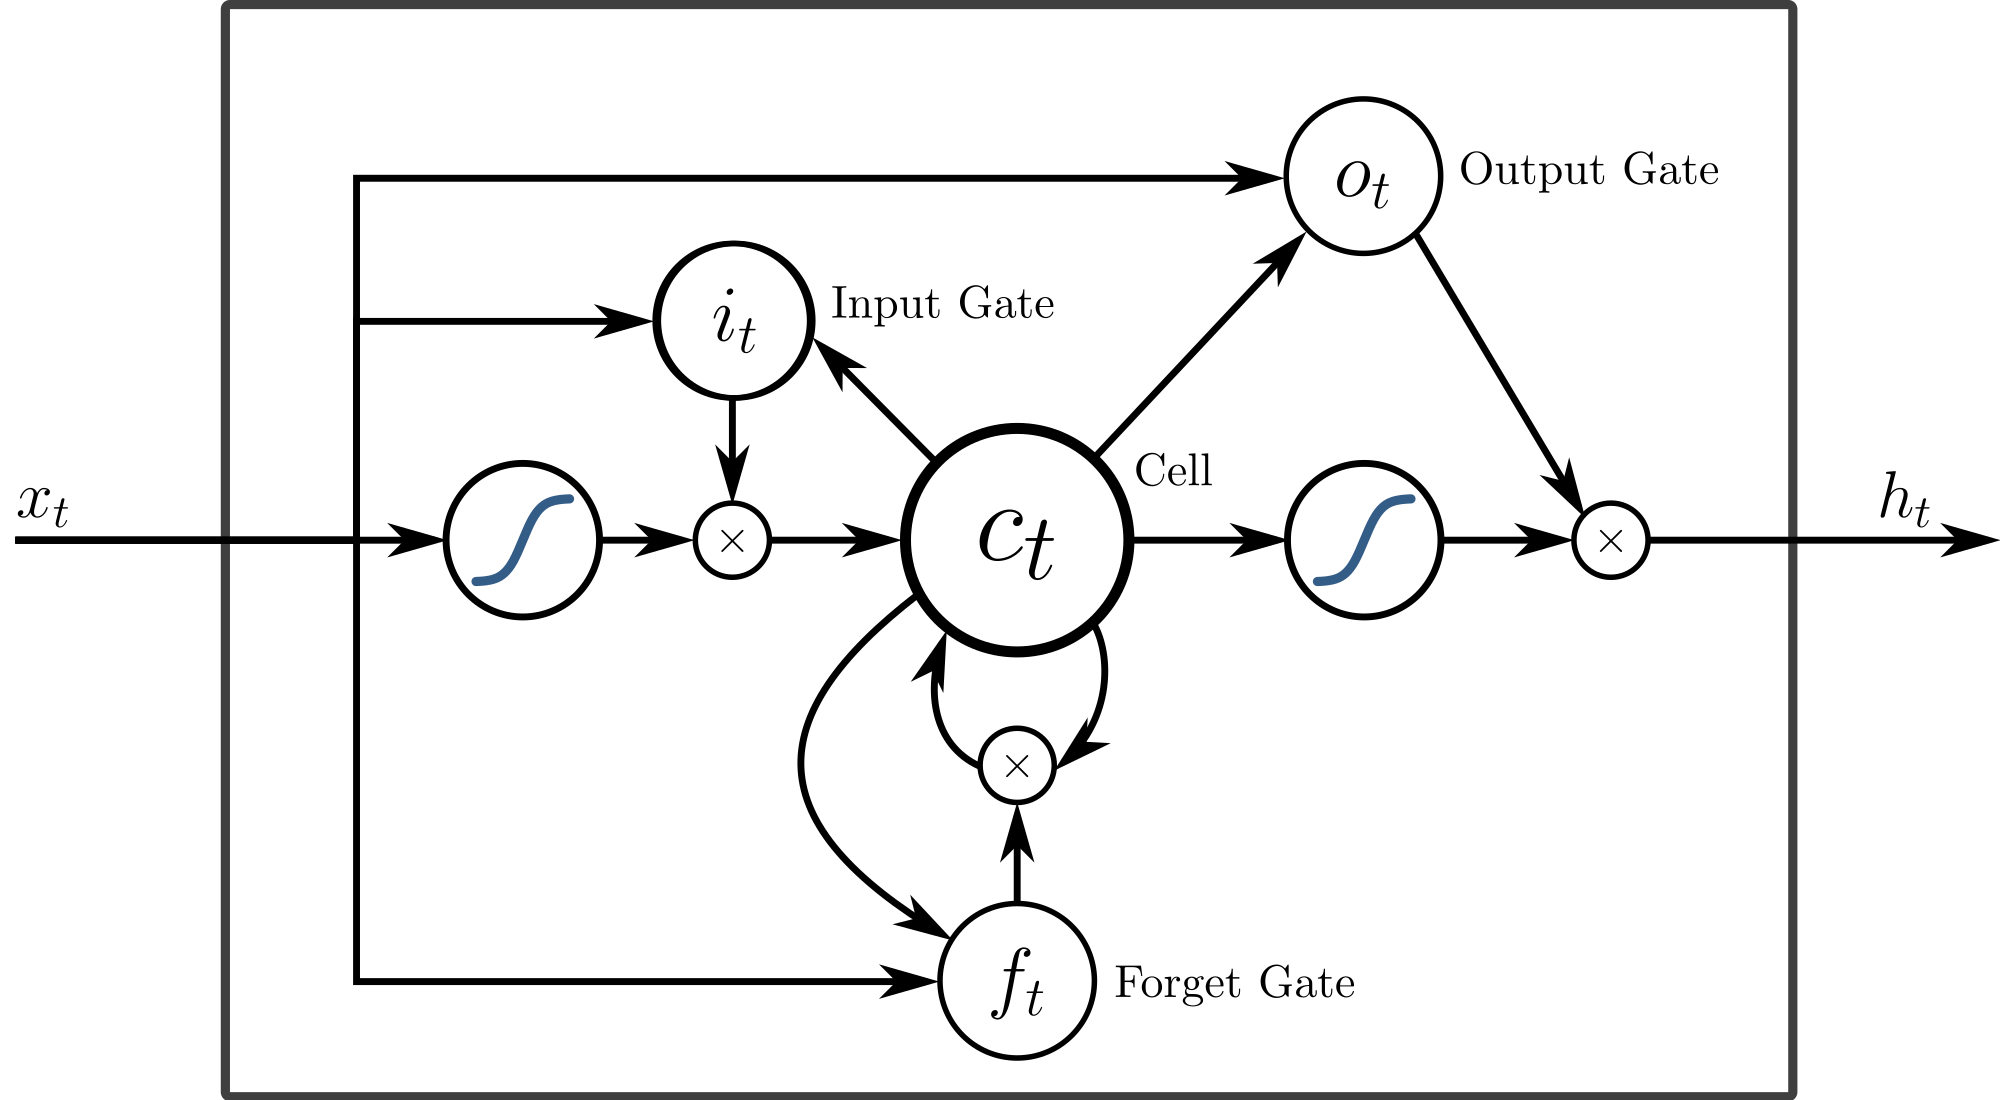
\includegraphics[width=\textwidth]{images/LSTM.png}
	\caption{visualization of an LSTM. Figure taken from \protect\footnotemark} 
	\label{fig:LSTM}
\end{figure}

\footnotetext{\url{https://en.wikipedia.org/wiki/Long_short-term_memory}}

The mathematical equations describing the functionality of the LSTM can be found in equations \ref{eq:LSTM_first} to \ref{eq:LSTM_last}, where $W_x$ and $U_x$ represent the weight matrices for the input and recurrent connections respectively and $b_x$ the biases. $x$ can be either $i$ for the input gate, $f$ for the forget gate or $o$ for the output gate. $c_0$ and $h_0$ are initialized with 0, $\circ$ denotes the element-wise multiplication of vectors and $\sigma$ is the logistic sigmoid function $\sigma(x) = \frac{1}{1 + \exp(-x)}$.

\begin{align}
	f_t &= \sigma_g(W_f x_t + U_f h_{t-1} + b_f) 
	\label{eq:LSTM_first}\\
	i_t &= \sigma_g(W_i x_t + U_i h_{t-1} + b_f) \\ 
	o_t &= \sigma_g(W_o x_t + U_o h_{t-1} + b_f) \\ 
	c_t &= f_t \circ c_{t-1} + i_t \circ \sigma_c (W_c x_t + U_c h_{t-1} + b_c) \\
	h_t &= o_t \circ \sigma_h (c_t)
	\label{eq:LSTM_last}
\end{align}


Importantly, the LSTM does not have the vanishing gradient problem, since it can store information over time intervals of arbitrary length. The experiments in this paper are therefore conducted with LSTMs. \\
A network can have multiple LSTMs in its hidden layer to process more complex information. The number of LSTM units per layer is called hidden size. Additionally, multiple LSTM units could also be combined sequentially. This is then called stacked LSTM. \\
In general, LSTM networks currently outperform most other architecture on sequential data and are also used for all experiments in this work. 

\section{Dynamic Time Warping (DTW)}
\label{section:DTW}

Dynamic time warping (DTW) is an algorithm designed to measure the distance between sequences that could vary in speed, frequency or other measures. If, for example, the similarity between two slightly shifted sinusoidal with the same frequency was to be determined, a standard approach, i.e. a mean squared error, might result in a numerically high difference even though the functions are very similar. To prevent this the DTW algorithm calculates the differences between the sequences for all values in the first sequence for every value in the second. This results in a 2D matrix of distances between the two sequences. To determine the distance a mean squared error is chosen. To find the DTW distance the path following the lowest costs starting at $(0,0)$ and ending at $(n,n)$ is chosen. The sum of the values along the path are the final result of dynamic time warping. An algorithm in pseudo code can be found in algorithm \ref{alg:DTW}


\begin{minipage}[right]{0.9\linewidth}
	\begin{algorithm}[H]
	\SetKwInOut{Input}{Input}
	\SetKwInOut{Output}{Output}
	
	\Input{\;
		$s_1:$ array[0..n],\; 
		$s_2:$ array[0..m]
		}
	\Output{\;
		DTW distance between $s_1$ and $d_2$}
	\underline{DTWDistance} $(s_1, s_2)$:\;
	\;
		DTW := array [n,m] 	(initialize array) \;
		\;
		DTW[0,:] := inf		(first column set to infinity) \;
		DTW[:,0] := inf		(first row set to infinity) \;
		DTW[0,0] := 0		(first value set to 0) \;
		\;
		\For{ i := 0 to n}{
			\For{j := 0 to m}{
				cost := d(s1[i], s2[j])		(calculate distance between points) \;
				DTW[i,j] := cost + min(DTW[i-1, j],    (insertion) \;
							DTW[i, j-1],   (deletion) \;
							DTW[i-1, j-1]) (match) \;
				}
			}
		\Return(DTW[n,m]))		
	\caption{dynamic time warping algorithm in pseudo code. $n,m$ represent the length of sequence 1 and 2.}
	\label{alg:DTW}
\end{algorithm}
\end{minipage}


Since the calculation requires taking the distance between all points for each point the resulting complexity is quadratic for sequences of the same length. To reduce computational complexity and therefore save time by not computing entries, that are likely irrelevant, in this paper the FastDTW algorithm was chosen. FastDTW has linear time complexity and comes at the cost of potentially slightly worse results. 

\section{Self-Organizing Feature Map (SOM)}
\label{section:SOM}

A self-organizing feature map (SOM) is used to produce low-dimensional (2D in this case) representations of the input space, usually called a map. A SOM is an artificial neural network that uses unsupervised learning and applies competitive learning instead of error-correction learning (like backpropagation) for the dimensionality reduction. Conceptually, a SOM unfolds the high-dimensional input space into a low-dimensional map, preserving the topological properties of the input, i.e. neighboring vectors in the input should also be neighbors in the output. \\ 
The map consists of multiple units to which weights are assigned at random in the beginning. After that a random vector is chosen from the training data and the best matching unit (BMU) of all weights is found, i.e. the unit with the smallest distance to the training sample. The neighborhood of the BMU is calculated. This means finding other units that are close to the BMU according to our chosen neighborhood function. After the neighborhood is determined the winning weight, i.e. the BMU is rewarded with becoming more like the sample vector. Neighboring units are also rewarded but to a lesser extend. In general, the higher the distance to the BMU the lower the reward for that weight. For this work a two dimensional Gaussian was chosen as the neighboring function. After repeating that process many times the average distance of every weight to their neighbors can be calculated and plotted. This is the easily visualized map that the SOM got its name from and which can be seen in multiple presentations of the experimental results in later sections. 

\section{k-Means Clustering}
\label{section:k-means_clustering}

The k-means clustering algorithm is used to find clusters of data points with high similarity in a given dataset. In this case the property to be compared is the Euclidean distance of the sequences. More specifically, the algorithm consists of two steps:\\
(1) Assignment: assign each data point to the cluster with the lowest euclidean distance to that point, i.e. the nearest mean of the cluster. \\
(2) Update: compute the new means to be the centers of the clusters. \\
If the assignments no longer change, the algorithm has converged. However, it is not necessary that the algorithm converges, since situations can arise in which the algorithm flip flops between two different states. Therefore the number of iterations in this paper is static and the final state needs to be taken as an approximation towards the real best state. In this paper the number of iterations was chosen to be high enough that SOMs for test samples did not change further. 
% Main chapter 3:
% Inverse classification using generative models
\chapter{Inverse Classification using Generative Models}
\label{chap:ICGM}

The main innovation of this paper is inverse classification using generative models. This means to first train a generative model to learn to generate sequences. In the second step this model is then used to inversely classify data by generating sequences with an input vector. The sequences are then compared to the target and the input vector is iteratively adapted through gradient based methods. A more detailed explanation of the two step process can be found in the following two sections.

\section{Sequence Generation}

A recurrent neural network with LSTMs is trained to generate sequences from class inputs. The classes are represented as one-hot vectors, i.e. vectors where one entry is one and all others are zero. The model gets the class information only in the very first timestep, being fed zero values for the rest. The model generates one part of the sequence at every point in time, not a one shot at the end. The sequences generated in this paper are two dimensional and represent the coordinates of a handwritten character trajectory. In principal every generative network could be used to inversely classify but since sequential data are being used, a recurrent model seemed appropriate. A graphical depiction of the process can be found in figure \ref{fig:generative_model}.

\begin{figure}[!htb]
	\centering
	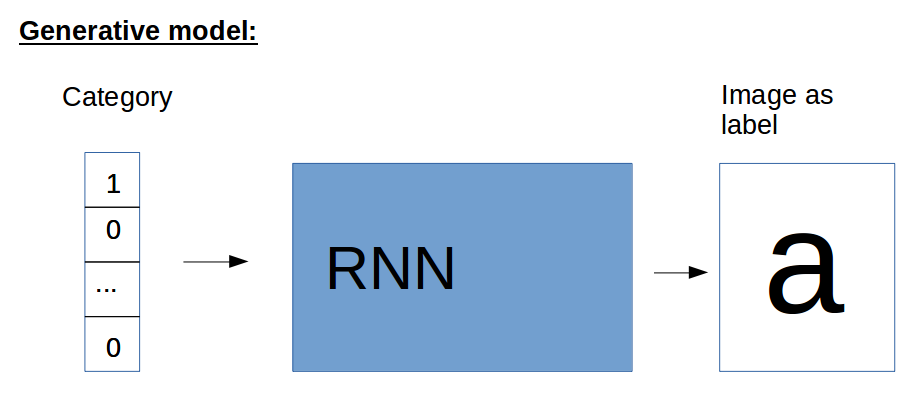
\includegraphics[width=\textwidth]{images/generative_model.png}
	\caption{Depiction of the sequence generation.}
	\label{fig:generative_model}
\end{figure}

\section{Inverse Classification}

The fully trained generative model is now used for inverse classification. Importantly, during the entire classification process the network weights are not changed. The success of the classification relies only on the concepts learned during the generative training. To classify a given target sequence, a character is generated. Since there is no prior information which character the target might be, the first generation is always performed from a uniformly distributed input vector. The resulting sequence is then compared to the sequence representing the target and an error is calculated. The gradient of the first layer of the network with respect to that error is then calculated and the uniformly distributed vector can be adapted proportional to the gradient. This process is done multiple times either until the input converges towards a static vector or the classification process is stopped after a given amount of steps. In the optimal case the input converges towards the one-hot vector representing the class of the target. Mathematically speaking, the inverse classification can be thought of as the inverse function to the generation. This implies that $f^{-1}(f(x)) = x$ if the inverse classification process works optimal, where $f(x), f^{-1}(x)$ denote the generative network and inverse classification respectively. A graphical interpretation of the process can be found in figure \ref{fig:inverse_classification}. 

\begin{figure}[!htb]
	\centering
	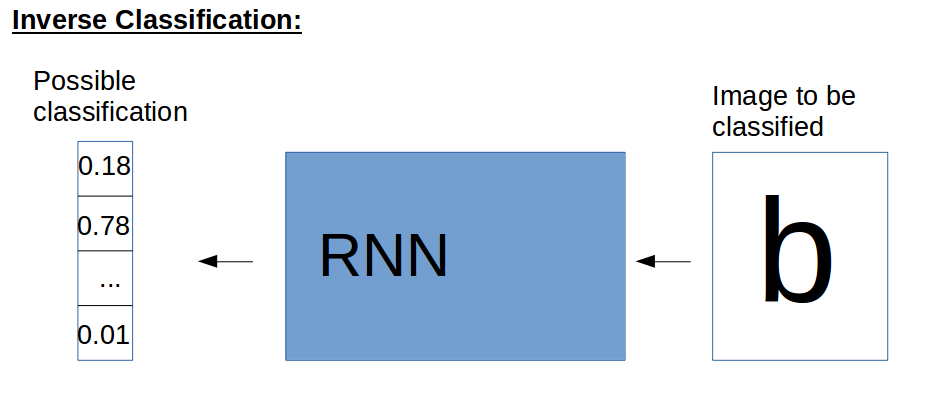
\includegraphics[width=\textwidth]{images/inverse_classification.png}
	\caption{Depiction of the inverse classification.}
	\label{fig:inverse_classification}
\end{figure}


% Main chapter 4:
% Experiments
\chapter{Experiments and Results}
\label{chap:Experiments}

In the following chapter multiple different techniques are implemented and tested.

\section{Setup}

To make this work reproducible the following section gives a full description of the setup used in the experiment.

\subsection{Data}
	The data are handwritten digits taken from the UCI Machine Learning Repository Character Trajectories Data Set from 2008 \cite{uci2013}. 
	It contains only characters that can be written in a single stroke, leading to 20 different classes with 2858 example characters in total. The six remaining letters of the alphabet are left out since they cannot be written within a single stroke. \\
	Originally the digits are saved with x- and y- delta values, i.e. the difference between two following points and a z-value representing the pin pressure used during the process of writing. For this work the cumulative sum of the deltas are taken to get the absolute coordinates for the training and the values for pin pressure are removed. A network trained on deltas instead of coordinates performed worse and the pin pressure did not add predictive value.
	The data are padded with the last coordinate such that all have the same length but no information is added or removed. 
	Additionally, the individual characters are standardized globally with mean 0 and standard deviation 1. Standardization leads to slightly better predictions. 
	For every experiment the data are split into 80\% training and 20\% test data. The test data are not used for validation during training but only after the training is finished.
	Lastly, it should be noted that the characters are often hard to distinguish even for humans. In figure	\ref{fig:hard_characters}
	a cherry-picked 'u' is depicted on the left and a cherry-picked 'w' on the right. This fact makes the classification more complicated. 
	
	\begin{figure}[!htb]
		\centering
		\begin{tabular}{cc}
			\subfloat[]{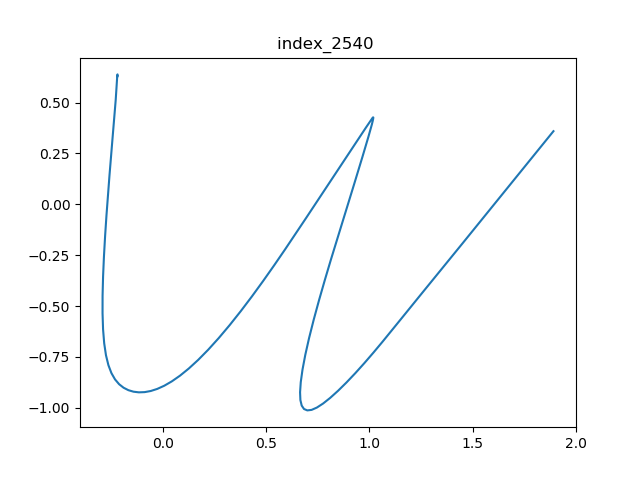
\includegraphics[width=5cm]{images/char_u_index_2540.png}} 
			& \subfloat[]{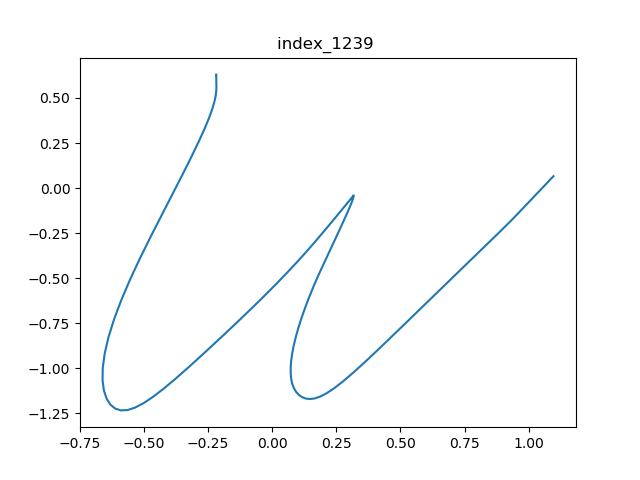
\includegraphics[width=5cm]{images/char_w_index_1239.png}}
		\end{tabular}
		\caption{On the left the character 'u' and on the right the character 'w' is depicted as they are found in the data set. Since they are rather similar in look the network might have additional difficulties separating them accordingly.}
		\label{fig:hard_characters}
	\end{figure}

\subsection{Generative Model}
\label{subsec:generative_model}
	As a model a sequential model of an LSTM with hidden size 205 and a fully connected (FC) layer with two neurons is used. The FC layer makes sure that during every timestep one coordinate of the sequence representing a character is generated. As activation functions we use \textit{$\tanh$} for the LSTM layer and a linear function for the FC layer. \\
	Different numbers for the amount of LSTM cells were tested and 205 seemed to be optimal, since smaller numbers did not generate high quality characters and bigger numbers did not improve results significantly. A graphical description of the model can be seen in figure \ref{fig:generative_model_details}. \\
	The network is given a one-hot vector in the first time step and only given vectors of zeros afterwards during the generative process. This makes sure that the network is really generating the sequence with only one piece of information in the beginning, preventing it from regaining the class information at later time steps.\\
	The training process uses a fixed number of epochs, a validation split of 0.2/0.8 and the model with the best validation error is chosen. The number of epochs is chosen in a way that ensures convergence and is evaluated with regards to the validation loss. As an optimizer Adam with standard values of $\alpha = 0.0001, \beta_1 = 0.9, \beta_2 = 0.999$ and $\epsilon = 10^{-8}$ is used. For further information on Adam see \cite{AdamKingmaB14} or algorithm \ref{alg:Adam}.\\
	There are always five instances of a model with exactly the same parameter values trained and their metrics aggregated since the variance between training sessions was high in early trials. 
	To train the model keras (\cite{chollet2015keras}) is used as a wrapper with a tensorflow (\cite{tensorflow2015-whitepaper}) backend. 
	
\begin{figure}[!htb]
	\centering
	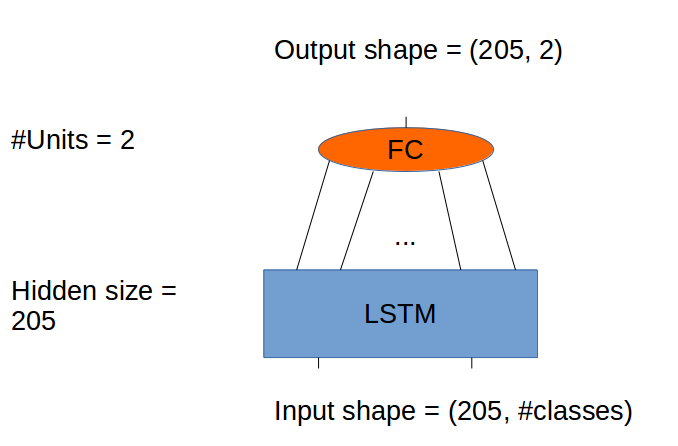
\includegraphics[width=0.7\textwidth]{images/generative_model_details.png}
	\caption{Implementation details of the generative model. LSTM with hidden size of 205 combined with a fully connected layer with 2 units generating 2D sequences of length 205, since this is the number of timesteps used. This model is not unfolded over time.}
	\label{fig:generative_model_details}
\end{figure}
	
	
\subsection{Inverse Classification}
\label{subsec:inverse_classification}
	For the inverse classification the already trained generative forward model is used. Every inverse classification is initialized with a uniformly distributed input vector and then adapted through the method described in chapter \ref{chap:ICGM} over 200 iterations. A fixed amount of iterations does not ensure that every classification converges but some were either converging towards a wrong class or flip-flopping between decisions making loss-based stopping impossible. During every iteration the new vector is clipped between 0 and 1 and then normalized to force convergence towards a one-hot vector.
	For the generative model the Adam optimizer (algorithm \ref{alg:Adam} or \cite{AdamKingmaB14}) was used for optimization with a learning rate of 0.05. All other values were the standard values already described in the previous section. This is a very high learning rate compared to the usual value of 0.001 but consistently provided the best results, probably due to the low number of iterations that was chosen. A higher number of iterations does not seem to fit the task though, since classification should not take too long for practical applications. An implementation of the algorithm in pseudo code can be found in algorithm \ref{alg:Adam}.
	
	\begin{algorithm}
		\SetKwInOut{Input}{Input}
		\SetKwInOut{Output}{Output}
		
		\Input{\;
			   $\alpha$  (Stepsize),\; 
			   $\beta_1, \beta_2$ (Exponential decay rates for the moment estimates),\;
			   $f(\theta)$ (Objective function with parameters $\theta$),\;
			   $\theta$ (initial parameter vector),\;
			   $\epsilon$, \;
			   $n_i$ (number of iterations)}
		\Output{\;
			$\theta_t$ (resulting parameters)}
		\underline{function Adam} $(\alpha,\beta_1, \beta_2, f(\theta), \theta, n_i)$:\;
		$m _0 = 0$ (initialize 1st moment vector)\;
		$m_1 = 0$ (initialize 2nd moment vector)\;
		$t = 0$ (initialize timesteps)\;
		\While{$t < n_i$}{
				$t = t + 1$\;
				$g_t = \nabla_\theta f_t(\theta_{t-1})$ get gradients for first layer w.r.t the loss function\;
				$m_t = \beta_1 \cdot m_{t-1} + (1 - \beta_1) \cdot g_t$ (Update first moment estimate)\;
				$v_t = \beta_2 \cdot v_{t-1} + (1 - \beta_2) \cdot g_t^2$ (Update second moment estimate)\;
				$\theta_t = \theta_{t-1} - \alpha \cdot \frac{m_t}{\sqrt{v_t + \epsilon}}$ (Update parameters)
			}
		\Return($\theta_t$) (resulting parameter)
		\caption{Adam algorithm with parameters $\alpha = 0.05, \beta_1 = 0.9, \beta_2 = 0.999, \epsilon = 10^{-8}$ and $n_i = 200$. The Objektive function is the MSE loss and the parameters are only the input vector that is adapted through inverse classification.}
		\label{alg:Adam}
	\end{algorithm}
	
	
	For the inverse classification also all five instances of the model with same parameters are used to be able to provide an estimate for the robustness of a model. To avoid confusion for the rest of the paper the terminology `instances of a model' is used to describe a model with exactly the same parameter settings independently trained on the exact same data but for multiple times.

\subsection{Metrics}
	To evaluate the quality of our model and the changes made during the experiments, two main metrics are established. \\
	With the first metric the quality of the model with given features is measured. It is essentially an exploration of the latent space of the model. For that a test space of all possible combinations of values ranging from 0 to 1 with step size n is created. This leads to a space of size $(n+1)^d$ where $d$ is the dimensionality. For each vector of the test space the model predicts the sequence and saves the distance of the generated sequence to a given target sequence. As a distance metric fast dynamic time warping (fastDTW) is chosen. A simple root squared mean error (RMSE) can also be used but produces worse results for trajectories as explained in section \ref{section:DTW}. The distances are then represented as heat maps for two dimensions and projected down from higher dimensions to 2D with the usage of self-organizing maps (SOMs). Notably, for higher dimensions only the vectors are explored that sum up to 1 since an entire analysis of the latent space would need too much computational power.\\
	The extensive exploration of the latent space within this work is due to the finding that the quality of the latent space directly and strongly influences the accuracy of the inverse classification. This implies that a clean clustering of characters in the latent space is a strong predictor for a good result in the inverse classification. It also implies that systematic deviations from a cluster can be solved in later experiments.\\
	Lastly, it needs to be pointed out that the quality of the generated characters is not quantitatively compared between the different type of networks but rather pointed out qualitatively, i.e. that a network produces high amounts of one particular character even if the vector producing it has another entry that is higher than for the produced result. \\
	The second metric regards the primary part of this research work, the inverse classification. To test how well a model performs the entire test set is classified and the accuracy of the classification calculated. The accuracy is determined by rounding the result to the closest one-hot vector and comparing it to the real target. To get an estimate of the distance between the inversely classified vector and the target their root mean-squared error is calculated additionally. \\
	For every experiment two, four and 20 dimensions are being tested. Dimensions in this case simply means the number of characters that the network was trained on, since directly going for all 20 characters turned out to be too complex of a task in many cases. 
	
\section{Naked Model}

For the first experiment the model described in subsection \ref{subsec:inverse_classification}
is used without any additions. 

\subsection{Two Dimensions}

At first the performance of the model with no further additions is tested. All five instances are tested against each other through the comparison of their heat maps. The heat map represents the DTW-distance from a generated letter to a given target character. In the optimal case a clean cut line on the diagonal representing $x=y$ could be seen since that marks the border of vectors where  the maximal value is closest to the corresponding one-hot vector. In the first five figures the distance to the character `a' is depicted while in the 6th the distance to a given `b' for the first model can be seen. This is used to show that the heatmaps from one model are exactly mirrored when different letters are chosen. This is an important finding because it shows that the model has learned abstract concepts of letters that correspond to different regions in latent space. The heat maps can be seen in figure \ref{fig:2_naked}. \\ 
The naked model does perform suboptimal in two major ways. First, it is not very consistent between different models, resulting in more effort to get good results. Second, it is very far from the optimal border of the $x=y$ diagonal. This is especially unfortunate since it implies worse results for the inverse classification.  

\begin{figure}[!htb]
	\centering
	\begin{tabular}{ccc}
		\subfloat[]{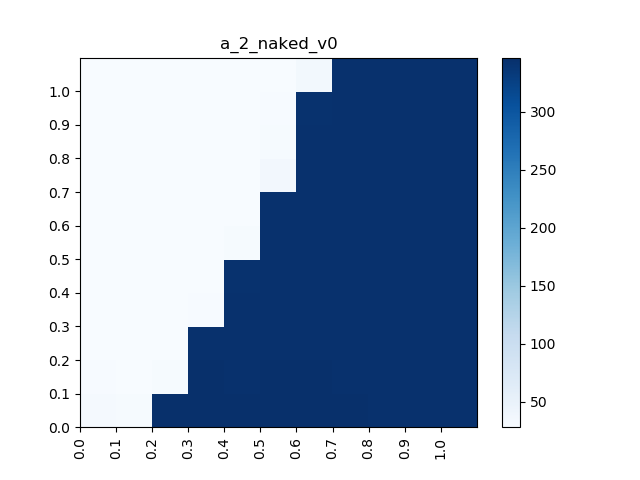
\includegraphics[width=5cm]{images/heat_maps/2_naked/a_2_naked_v0.png}} 
        & \subfloat[]{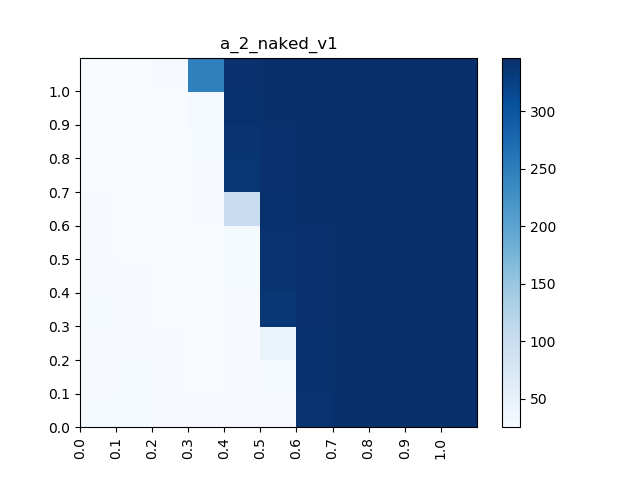
\includegraphics[width=5cm]{images/heat_maps/2_naked/a_2_naked_v1.png}}
		& \subfloat[]{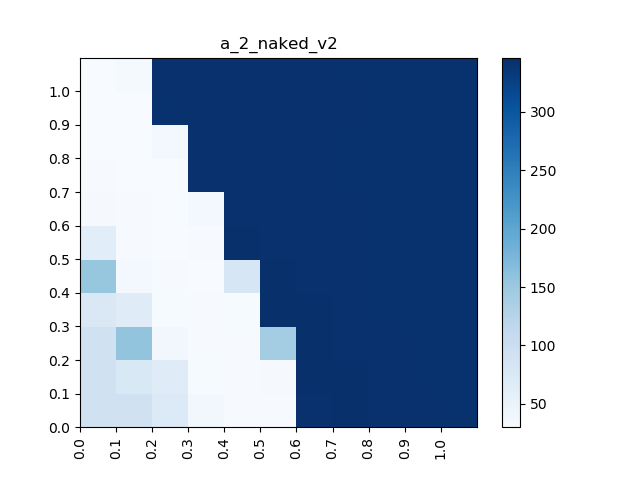
\includegraphics[width=5cm]{images/heat_maps/2_naked/a_2_naked_v2.png}} \\
		\subfloat[]{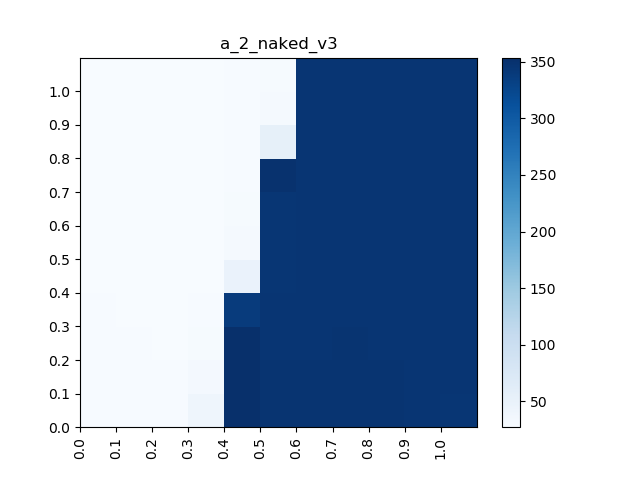
\includegraphics[width=5cm]{images/heat_maps/2_naked/a_2_naked_v3.png}}
		& \subfloat[]{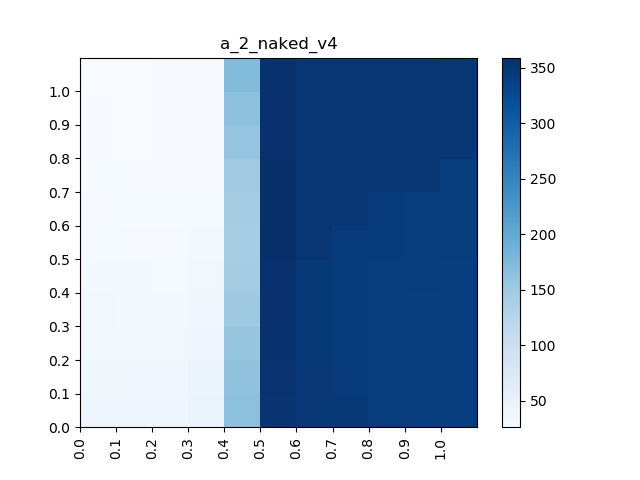
\includegraphics[width=5cm]{images/heat_maps/2_naked/a_2_naked_v4.png}} 
		& \subfloat[]{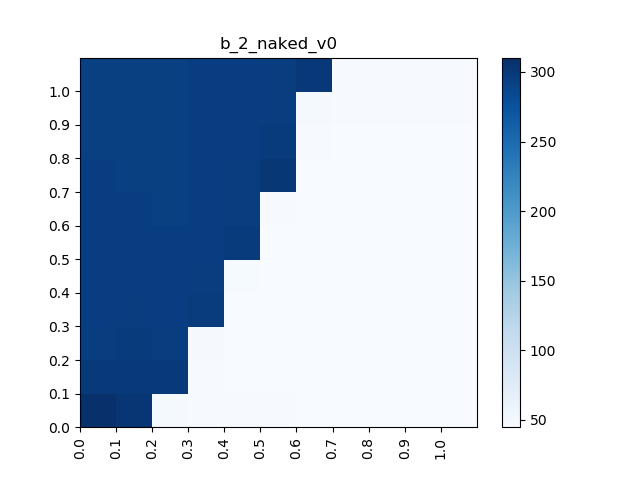
\includegraphics[width=5cm]{images/heat_maps/2_naked/b_2_naked_v0.png}}
	\end{tabular}
	\caption{ (a) - (e) represent the distance of the classification data to a given instance of the character `a' of five instances of the model with no additions that are independently trained on the same dataset. (f) shows the distance of the same instances as depicted in (a) to the character 'b'. }
	\label{fig:2_naked}
\end{figure}

After the exploration of the latent space the inverse classification is analyzed. For this the Inverse Classification algorithm as described in chapter \ref{chap:ICGM} is performed on all test characters. Note that they are previously unknown to the trained network. In table \ref{table:2_naked} the models and their respective accuracy and root mean squared error (RMSE) are depicted. All values are rounded to 2 decimal digits. 

\begin{table}[!htb]
	\centering
	\caption{Results for the 2D models without additions. The first five rows represent the accuracy and RMSE for each instance of the model while the last two show mean and standard deviation for each respective category.}
	\begin{tabularx}{\textwidth}{ X  X  X }
		\hline
		model & accuracy & RMSE \\ 
		\hline
		2\_naked\_v0 & 0.7 & 0.36\\
		2\_naked\_v1 & 0.57 & 0.44\\
		2\_naked\_v2 & 0.81 & 0.32 \\
		2\_naked\_v3 & 0.84 & 0.17 \\
		2\_naked\_v4 & 0.38 & 0.6 \\ 
		\hline
		mean & 0.66 & 0.38 \\
		standard deviation & 0.17 & 0.14 \\
		\hline
	\end{tabularx}
	\label{table:2_naked}
\end{table}

The average accuracy of 0.66 and error of 0.38 are better than a random guess which would result in a value of 0.5. There is rather high standard deviation of 0.17 regarding accuracy and 0.14 regarding the error between the models. Four out of five meet the burden of beating random guessing but  instance 4 is worse. Two additional observations are: a) accuracy and RMSE are highly correlated. This very likely implies that a good model not only makes correct predictions but also ones that are closer to the corresponding one-hot vector. b) There is a tendency that models which have heat maps closer to an optimal heat map have higher accuracy and lower error. Instance 2 seems to be an outlier given that significantly more than half of its latent space is occupied by representations of the character `b' making this result surprisingly good.

\subsection{Four Dimensions}

Another five different instances of the model with no addition were trained on a dataset with four different characters, i.e. `a', `b', `c' and `d'. Since a four dimensional heat map is not very clear, a self-organizing feature map is used to analyze the latent space for these models. Given that the figures coming from the SOM are quite large only selected SOMs and sometimes only certain aspects are reviewed. In figure \ref{fig:4d_naked_all}
the SOM for version 0 of the model without additions can be seen. The red vectors are the basis for the prediction and the blue characters the respective results. It is hard to identify the different aspects of the figure. The focus therefore lies on select insights. First, the latent space did not unfold itself into four regionally separated classes standing for the four characters. But still most cells only represent one character and multiple of the same classes create clusters with low average distances in certain parts of the map. Second, the character `a' and `c' are represented way more often than `b' and `d' even though their representation within the training set is uniformly distributed. For this model only four instances of each of the rarer characters can be found when 286 characters are represented in total. A majority of the bad results in the inverse classification is therefore likely due to the underrepresentation of `b' and `d' in the models latent space. Since figure \ref{fig:4d_naked_all} is hard to interpret, figure \ref{fig:4d_naked_a} shows the same map with only the character `a'. As can be seen, different clusters on the same cell or with low regional difference are formed. Often the vectors producing similar characters share certain properties, i.e. three vectors on the right edge of the map are all close to uniformly distributed and located on the same cell. Quantitatively the model performs better than guessing since all accuracies are over 0.25 and the  errors are lower than $[\frac{1}{4} (3*(0.25 -0)^2 + (0.25 -1)^2)]^{0.5} = 0.43$ as can be seen in table \ref{table:4_naked}. The average accuracy of the inverse classification of 0.49 makes sense in the context of the analysis of the latent space. The model mostly learned the concept of `a' and `c'. It therefore classifies all of these characters correctly, but all `b's and `d's are categorized incorrectly as one of the two others. The variance of classification is still very high with a value of 0.14. This implies that the model is still not very robust between different training sessions making it rather unusable for practical purposes.


\begin{table}[!htb]
	\centering
	\caption{Results for the 4D models without additions. The first five rows represent the accuracy and RMSE for each instance of the model while the last two show mean and standard deviation for each respective category.}
	\begin{tabularx}{\textwidth}{ X  X  X }
		\hline
		model & accuracy & RMSE \\ 
		\hline
		4\_naked\_v0 & 0.67 & 0.29 \\
		4\_naked\_v0 & 0.62 & 0.27 \\
		4\_naked\_v0 & 0.47 & 0.38 \\
		4\_naked\_v0 & 0.36 & 0.4  \\
		4\_naked\_v0 & 0.32 & 0.39 \\
		\hline 
		mean & 0.49 & 0.35  \\
		standard deviation & 0.14 & 0.05 \\
		\hline
	\end{tabularx}
	\label{table:4_naked}
\end{table}


\begin{figure}[!htb]
	\centering
	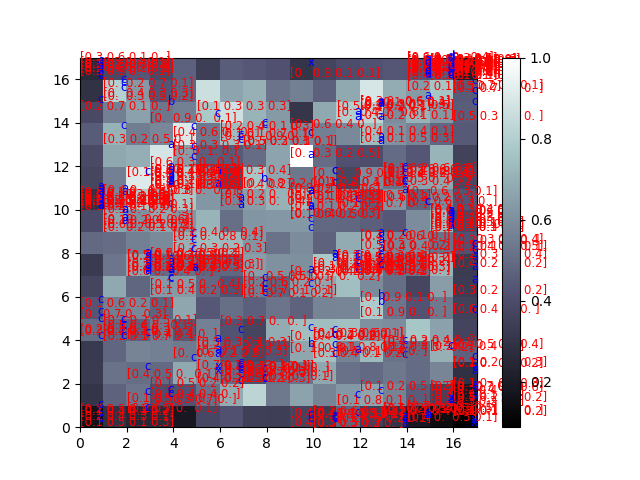
\includegraphics[width=\textwidth]{images/SOM_graphics/17x17_4d_naked_v0/all.png}
	\caption{SOM for version 0 of the model without additions trained on 4 characters. Red vectors are the bases for the prediction and blue characters are the result of the given prediction. The map in the background shows the average distances for each weight to their neighbors.}
	\label{fig:4d_naked_all}
\end{figure}

\begin{figure}[!htb]
	\centering
	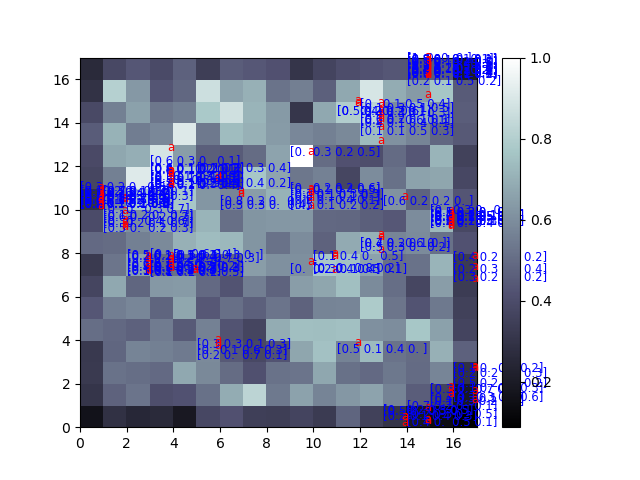
\includegraphics[width=\textwidth]{images/SOM_graphics/17x17_4d_naked_v0/a.png}
	\caption{SOM for version 0 of the model without additions trained on 4 characters. Only the letter 'a' is represented. Red vectors are the bases for the prediction and blue characters are the result of the given prediction. The map in the background shows the average distances for each weight to their neighbors.}
	\label{fig:4d_naked_a}
\end{figure}

\subsection{20 Dimensions}

Since our data has 20 different characters at the end of every experiment the same procedure as before is performed for 20 dimensions.


\begin{table}[!htb]
	\centering
	\caption{Results for the 20D models without additions. The first five rows represent the accuracy and RMSE for each instance of the model while the last two show mean and standard deviation for each respective category.}
	\begin{tabularx}{\textwidth}{ X  X  X }
		\hline
		model & accuracy & RMSE \\ 
		\hline
		20\_naked\_v0 & 0.39 & 0.19\\ 
		20\_naked\_v1 & 0.41 & 0.2 \\
		20\_naked\_v2 & 0.34 & 0.2 \\ 
		20\_naked\_v3 & 0.34 & 0.2 \\ 
		20\_naked\_v4 & 0.25 & 0.2 \\ \hline
		mean & 0.35 & 0.2\\
		standard deviation & 0.05 & 0.0\\
		\hline
	\end{tabularx}
	\label{table:20_naked}
\end{table}

As can be seen in table \ref{table:20_naked} the model has an accuracy of 0.39 which is significantly better than a random accuracy of 0.05. The average error of 0.19 is also better than a guessing error of $[\frac{1}{20}(19 \cdot (0-0.05)^2 + (1-0.05)^2)]^{0.5} = 0.22$. However, that difference is not really big implying that the model either does not predict correct results with high certainty or that it predicts incorrect results with high certainty leading to high errors. 

\section{Double Stacked LSTM}

\subsection{Two Dimensions}

In this section the addition of a second LSTM layer and the respective capability to classify is explored. After the suboptimal results seen in the previous chapter an additional layer might provide better representation and generalization of characters and therefore yield better results. The second layer has exactly the same specifications as the layer in the single-layer models did, i.e. 205 hidden units and a \textit{$\tanh$} activation function. Every other part of the model is exactly the same as described in subsection \ref{subsec:inverse_classification}.

\begin{figure}[!htb]
	\centering
	\begin{tabular}{ccc}
		\subfloat[]{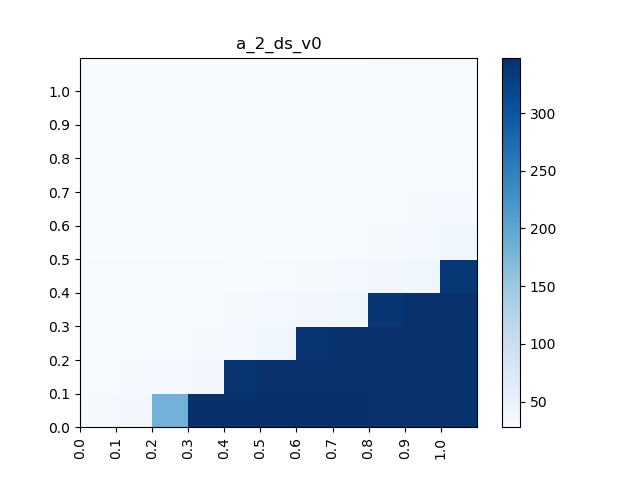
\includegraphics[width=5cm]{images/heat_maps/2_ds/a_2_ds_v0.png}} 
		& \subfloat[]{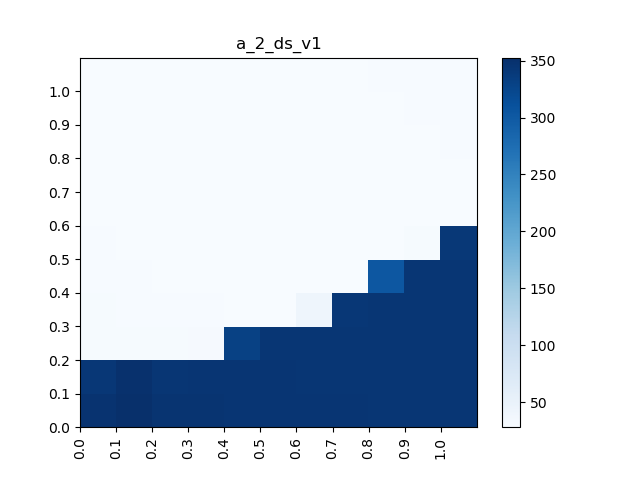
\includegraphics[width=5cm]{images/heat_maps/2_ds/a_2_ds_v1.png}}
		& \subfloat[]{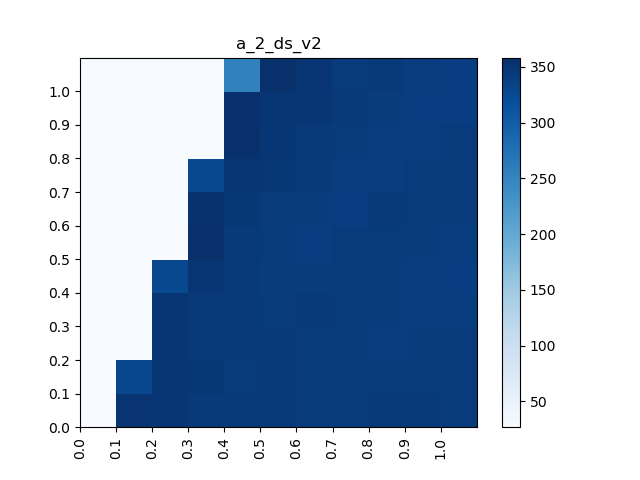
\includegraphics[width=5cm]{images/heat_maps/2_ds/a_2_ds_v2.png}} \\
		\subfloat[]{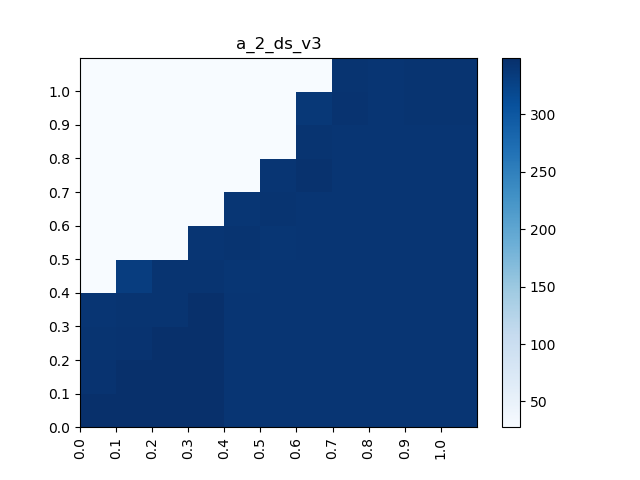
\includegraphics[width=5cm]{images/heat_maps/2_ds/a_2_ds_v3.png}}
		& \subfloat[]{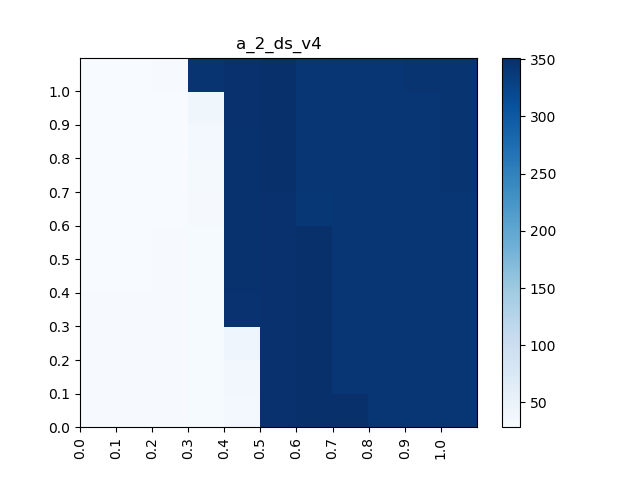
\includegraphics[width=5cm]{images/heat_maps/2_ds/a_2_ds_v4.png}} 
		& \subfloat[]{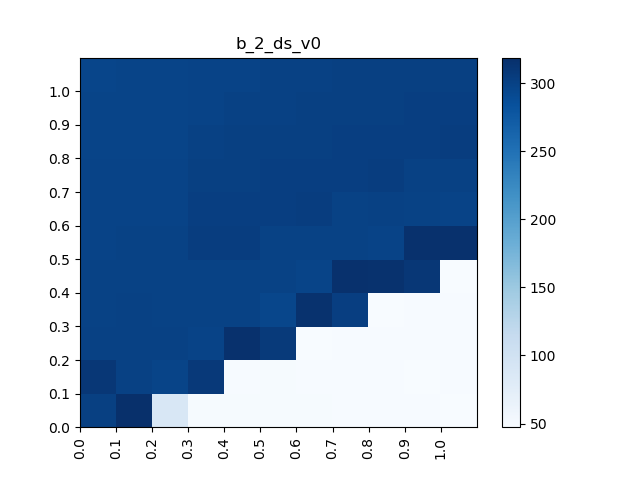
\includegraphics[width=5cm]{images/heat_maps/2_ds/b_2_ds_v0.png}}
	\end{tabular}
	\caption{ (a) - (e) represent the distance of the classification data to a given instance of the character 'a' of five instances of the model of double stacked LSTMs that are independently trained on the same dataset. (f) shows the distance of the same model as depicted in (a) to the character 'b'. }
	\label{fig:2_ds}
\end{figure}

The latent space is still very far from the optimal diagonal break and at least qualitatively no improvement on the single layer LSTM tested in the previous chapter. Qualitatively, as depicted in table \ref{table:2_ds}, the model is not better than the naked one, two of the five instances perform even worse than guessing. On average the mean accuracy and the mean error are very close to guessing without knowledge, i.e. a value of 0.5 for the inverse classification.

\begin{table}[!htb]
	\centering
	\caption{Results for the 2D models with a double stacked LSTM. The first five rows represent the accuracy and RMSE for each instance of the model while the last two show mean and standard deviation for each respective category.}
	\begin{tabularx}{\textwidth}{ X  X  X }
		\hline
		model & accuracy & RMSE \\ 
		\hline
		2\_double\_stacked\_v0 & 0.59 & 0.48 \\
		2\_double\_stacked\_v1 & 0.43 & 0.58 \\
		2\_double\_stacked\_v2 & 0.4 &  0.5 \\
        2\_double\_stacked\_v3 & 0.75 & 0.33 \\
		2\_double\_stacked\_v4 & 0.52 & 0.56 \\
		\hline 
		mean & 0.54 & 0.49 \\
		standard deviation & 0.12 & 0.09 \\
		\hline
	\end{tabularx}
	\label{table:2_ds}
\end{table}


\subsection{Four Dimensions}

The same analysis as for two characters is again done for four with the double stacked LSTM. As can be seen in table \ref{table:4_ds} the models vary very much. Model version 0 has an accuracy of 0.93 while version 4 has 0.3. On average the classification rate of the model with double stacked LSTMs is 0.65  beating the rate of the model without additions of 0.49. The reason for that can be found in figure \ref{fig:4d_ds_c}. Only the character `c' is represented since showing all would be too unclear. \\
As can be seen especially in the lower mid sections very big clusters of the same characters have formed within the latent space. Additionally the overlay between characters within the same regions is very low, i.e. borders are very sharp. This becomes especially visible when comparing the SOM of `c' to the SOM of `d' represented in figure \ref{fig:4d_ds_d}. The regions where `d's are clustered seem to be exactly the regions where `c's are not. The same holds true for `a' and `b' to a nearly similar extend but their SOMs are left out for the purpose of saving space. Additionally, the clusters represented in the SOM also share similarities. Many nodes, for example, seem to be defined through the size of the number at the third entry of the vector, i.e. the entry representing the class `c'. However, there are many exceptions to this trend, likely being one of the reasons why the model is not able to perform perfect inverse classification. 

\begin{figure}[!htb]
	\centering
	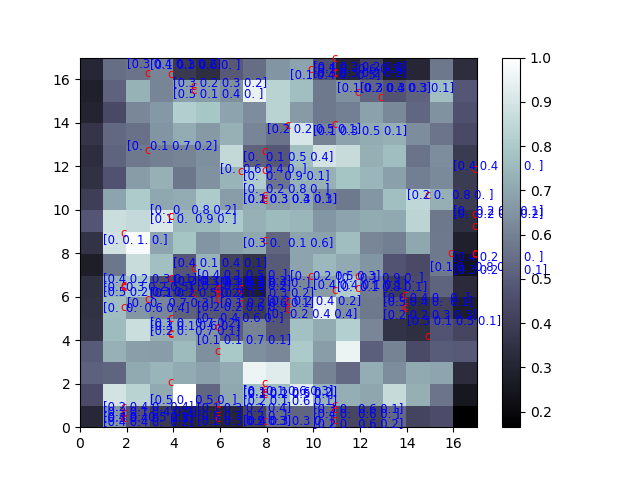
\includegraphics[width=\textwidth]{images/SOM_graphics/17x17_4d_ds_v0/c.png}
	\caption{SOM for version 0 of the model with the double stacked LSTMs trained on 4 characters. Only the letter `c' is represented. Red vectors are the bases for the prediction and blue characters are the result of the given prediction. The map in the background shows the average distances for each weight to their neighbors.}
	\label{fig:4d_ds_c}
\end{figure}

\begin{figure}[!htb]
	\centering
	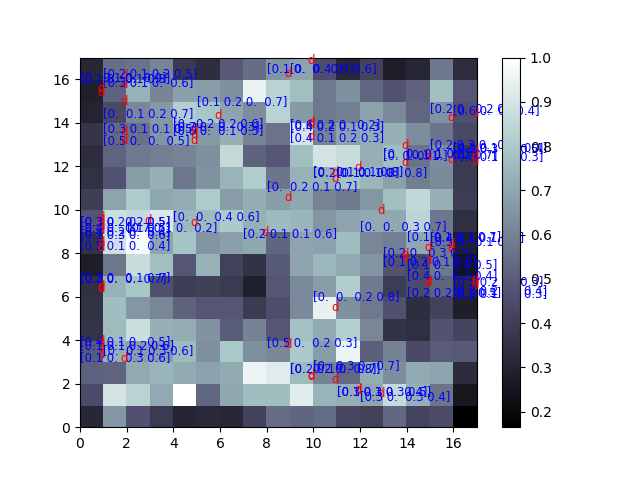
\includegraphics[width=\textwidth]{images/SOM_graphics/17x17_4d_ds_v0/d.png}
	\caption{SOM for version 0 of the model with the double stacked LSTMs trained on 4 characters. Only the letter `d' is represented. Red vectors are the bases for the prediction and blue characters are the result of the given prediction. The map in the background shows the average distances for each weight to their neighbors.}
	\label{fig:4d_ds_d}
\end{figure}


\begin{table}[!htb]
	\centering
	\caption{Results for the 4D models with double stacked LSTMs. The first five rows represent the accuracy and RMSE for each instance of the model while the last two show mean and standard deviation for each respective category.}
	\begin{tabularx}{\textwidth}{ X  X  X }
		\hline
		model & accuracy & RMSE \\ 
		\hline
		4\_ds\_v0 & 0.93 & 0.18\\
		4\_ds\_v1 & 0.66 & 0.28\\
		4\_ds\_v2 & 0.5 & 0.35\\
		4\_ds\_v3 & 0.87 & 0.25\\
		4\_ds\_v4 & 0.3 & 0.44\\
		\hline 
		mean & 0.65 & 0.3  \\
		standard deviation & 0.23 & 0.09 \\
		\hline
	\end{tabularx}
	\label{table:4_ds}
\end{table}


\subsection{20 Dimensions}


\begin{table}[!htb]
	\centering
	\caption{Results for the 20D models with double stacked LSTMs. The first five rows represent the accuracy and RMSE for each instance of the instance of the model while the last two show mean and standard deviation for each respective category.}
	\label{table:20_ds}
	\begin{tabularx}{\textwidth}{ X  X  X }
		\hline
		model & accuracy & RMSE \\ 
		\hline
		20\_ds\_v0 & 0.22 & 0.21\\
		20\_ds\_v1 & 0.29 & 0.21\\
		20\_ds\_v2 & 0.5  & 0.19\\
		20\_ds\_v3 & 0.31 & 0.2 \\
		20\_ds\_v4 & 0.31 & 0.2 \\
		\hline 
		mean & 0.32 & 0.2  \\
		standard deviation & 0.09 & 0.01 \\
		\hline
	\end{tabularx}
\end{table}

Results for the inverse classification of the double stacked LSTM models can be found in table \ref{table:20_ds}. The mean accuracy of 0.32 and the mean RMSE of 0.2 are comparable to the values of the naked models with 0.35 and 0.2 respectively. The standard deviation between models is also comparable with 0.09 and 0.01 for the double stacked and 0.05 and 0.0 for the naked one. The most likely conclusion is that the addition of a second stack of LSTM units is not an improvement for inverse classification, at least for this task.


\section{Addition of Noise}

After analyzing the model without additions and the double stacked LSTMs two problems emerged. Either the models did not learn one or two characters and therefore misclassified or they mapped very similar vectors to different classes. To make the latent space more clear cut a noise and a clip layer were introduced. This means that the generative network is still trained on one-hot vectors representing the classes but during every epoch for every instance Gaussian distributed noise with mean of 0 and different standard deviations is added on this input. The standard deviations start at 0.1 and are increased in steps of 0.1 over four separate experiments. Additionally the network has a clipping layer, meaning that every input has only entries between 0 and 1.

\subsection{Two Dimensions}

For two letters standard deviations of 0.1 - 0.4 are tested. The heat maps generated through the addition of noise during the training process can be seen in figure \ref{fig:2_noise}. A clear trend can be seen: the higher the standard deviation the closer the latent space is separated by the optimal $x = y$ diagonal. Additionally, the fuzziness of that border increases in the same process. This should imply that the rate of correct classifications increases for the models with these optimal latent spaces. \\

\begin{figure}[!htb]
	\centering
	\begin{tabular}{ccccc}
		\subfloat[]{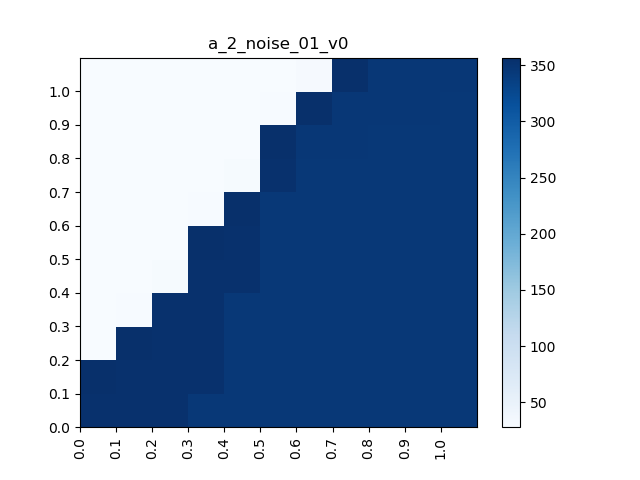
\includegraphics[width=3cm]{images/heat_maps/2_noise_01/a_2_noise_01_v0.png}} 
		& \subfloat[]{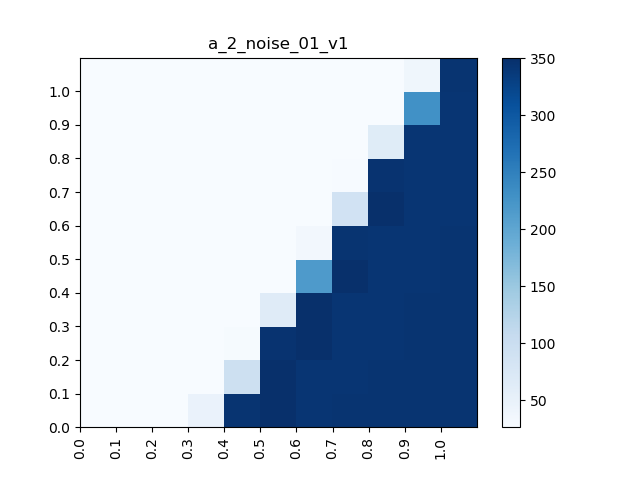
\includegraphics[width=3cm]{images/heat_maps/2_noise_01/a_2_noise_01_v1.png}}
		& \subfloat[]{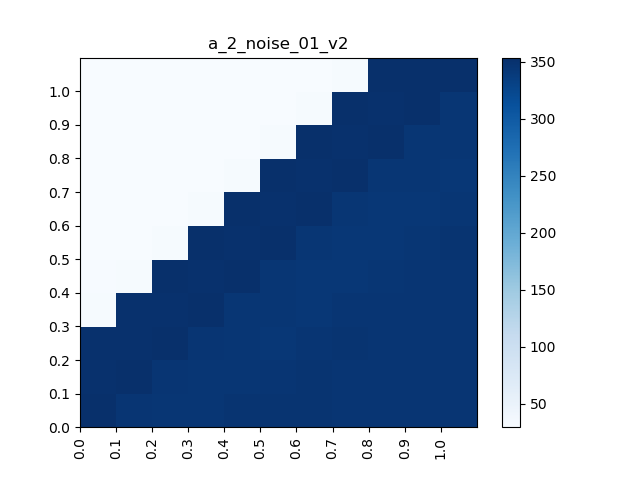
\includegraphics[width=3cm]{images/heat_maps/2_noise_01/a_2_noise_01_v2.png}} 
		&
		\subfloat[]{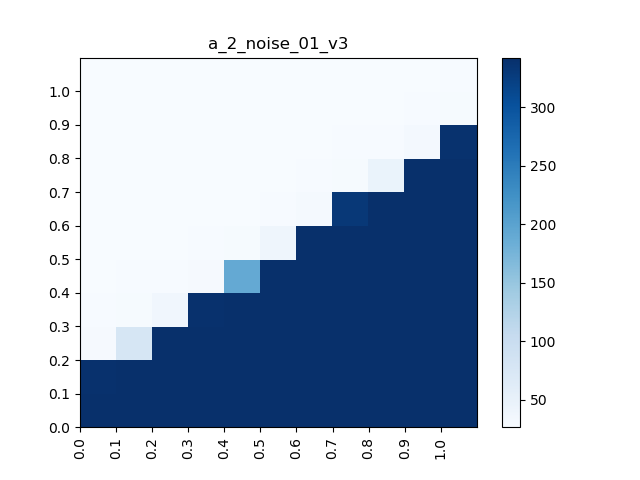
\includegraphics[width=3cm]{images/heat_maps/2_noise_01/a_2_noise_01_v3.png}}
		& \subfloat[]{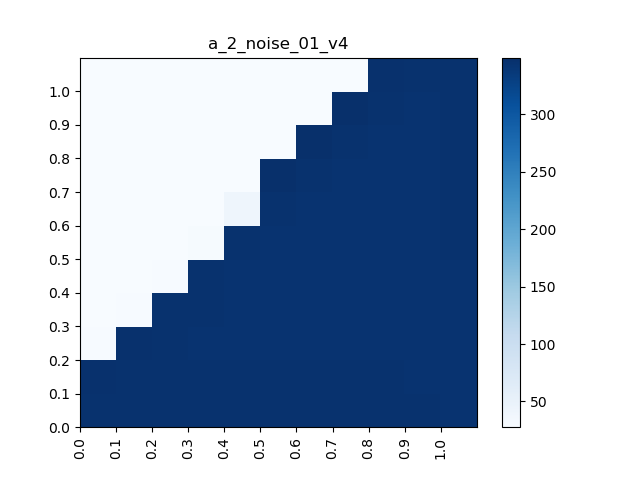
\includegraphics[width=3cm]{images/heat_maps/2_noise_01/a_2_noise_01_v4.png}} \\
		\subfloat[]{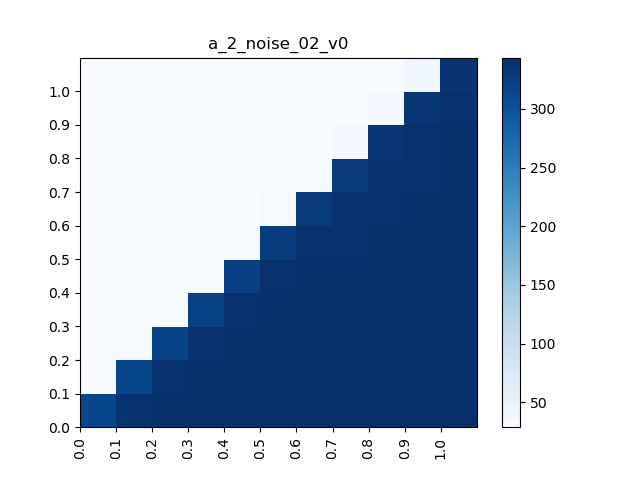
\includegraphics[width=3cm]{images/heat_maps/2_noise_02/a_2_noise_02_v0.png}} 
		& \subfloat[]{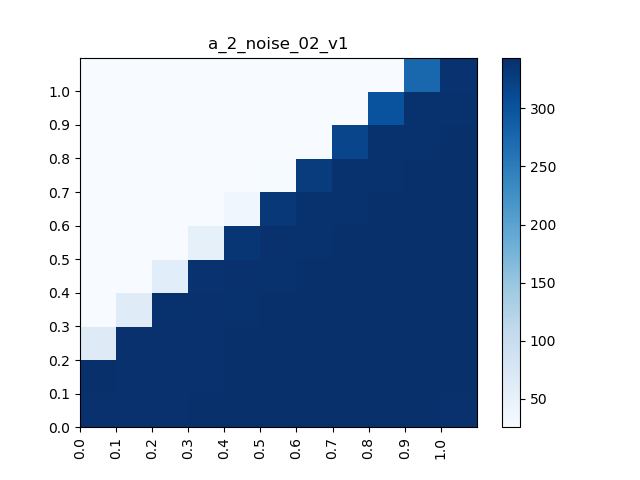
\includegraphics[width=3cm]{images/heat_maps/2_noise_02/a_2_noise_02_v1.png}}
		& \subfloat[]{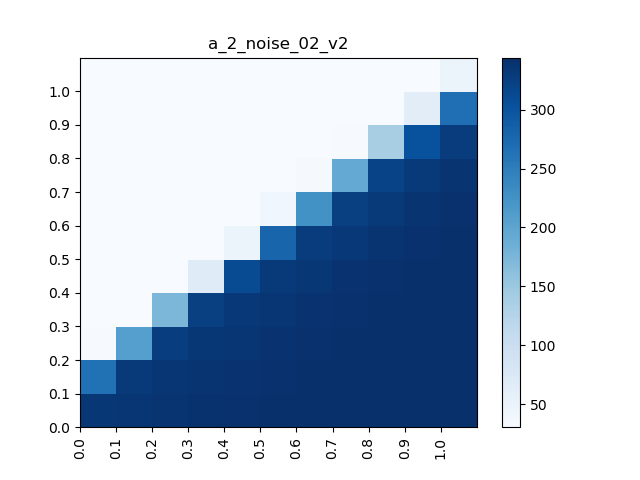
\includegraphics[width=3cm]{images/heat_maps/2_noise_02/a_2_noise_02_v2.png}}
		&
		\subfloat[]{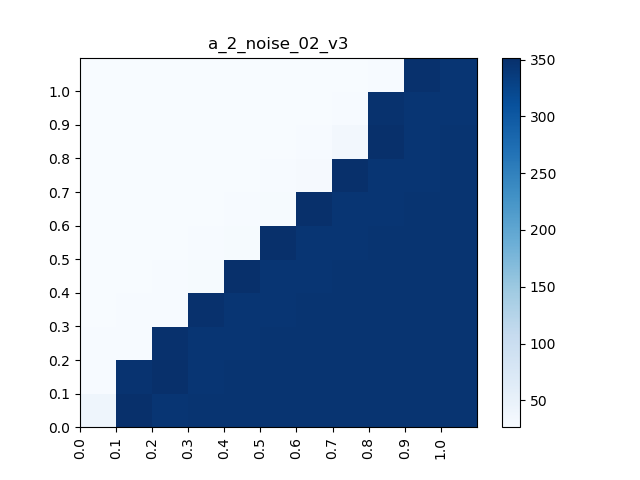
\includegraphics[width=3cm]{images/heat_maps/2_noise_02/a_2_noise_02_v3.png}}
		& \subfloat[]{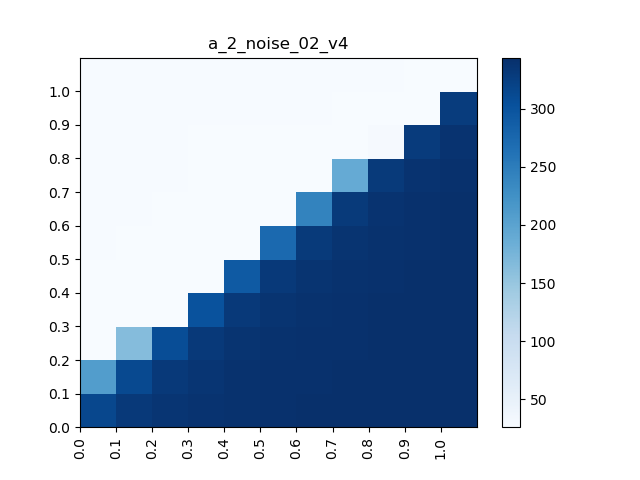
\includegraphics[width=3cm]{images/heat_maps/2_noise_02/a_2_noise_02_v4.png}}\\
		\subfloat[]{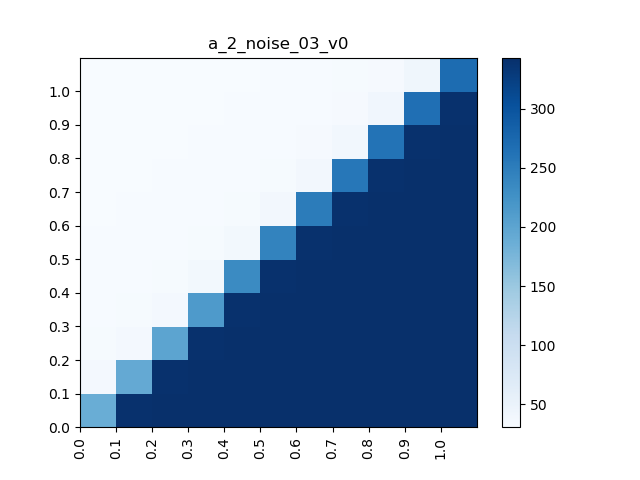
\includegraphics[width=3cm]{images/heat_maps/2_noise_03/a_2_noise_03_v0.png}} 
		& \subfloat[]{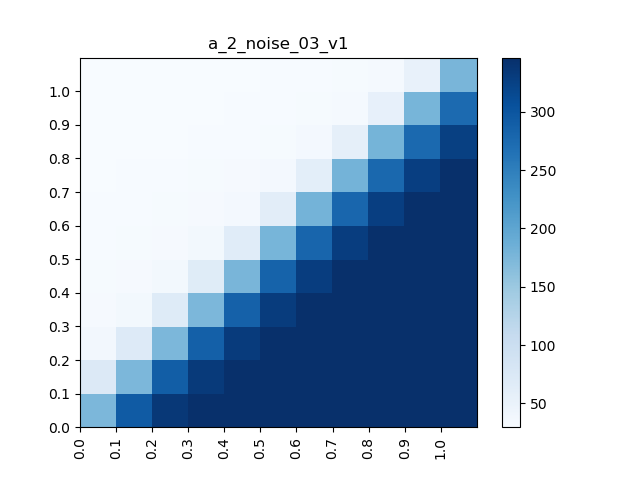
\includegraphics[width=3cm]{images/heat_maps/2_noise_03/a_2_noise_03_v1.png}}
		& \subfloat[]{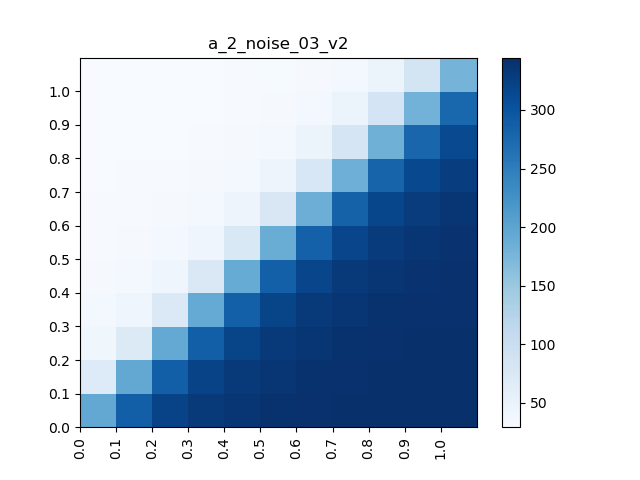
\includegraphics[width=3cm]{images/heat_maps/2_noise_03/a_2_noise_03_v2.png}} 
		&
		\subfloat[]{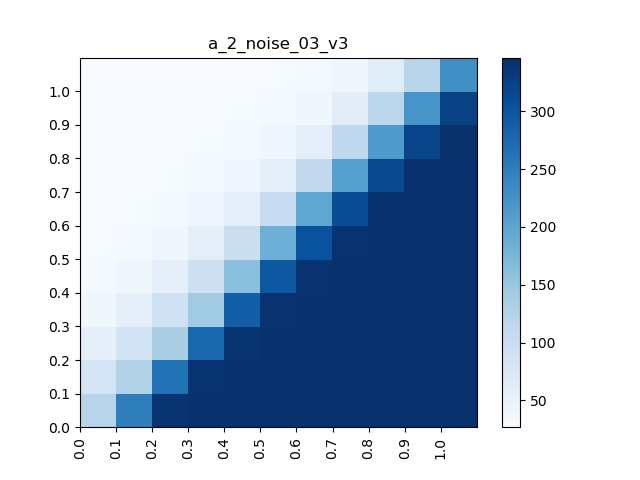
\includegraphics[width=3cm]{images/heat_maps/2_noise_03/a_2_noise_03_v3.png}}
		& \subfloat[]{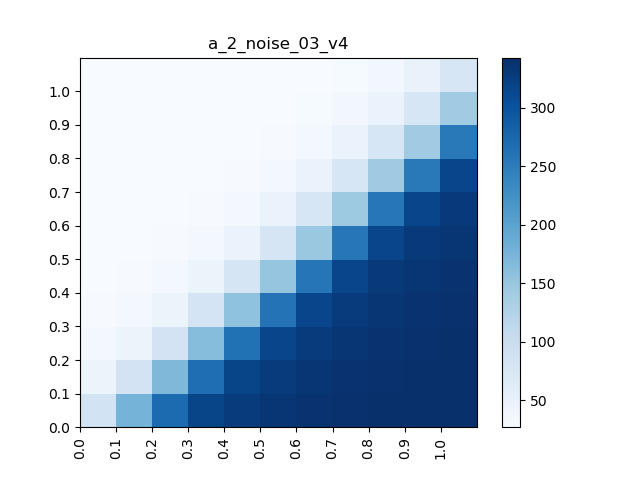
\includegraphics[width=3cm]{images/heat_maps/2_noise_03/a_2_noise_03_v4.png}} \\
		\subfloat[]{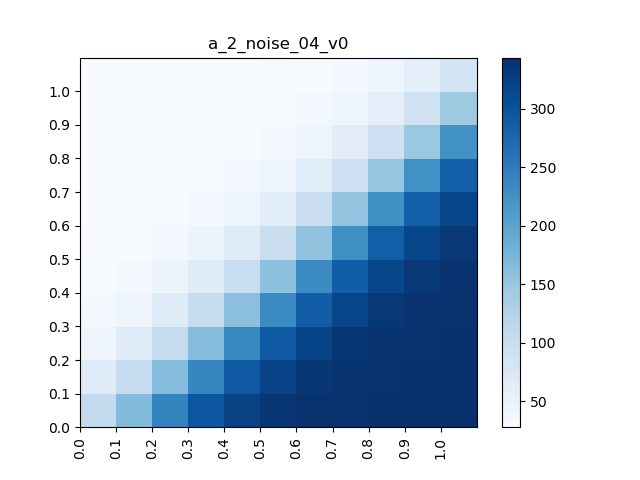
\includegraphics[width=3cm]{images/heat_maps/2_noise_04/a_2_noise_04_v0.png}} 
		& \subfloat[]{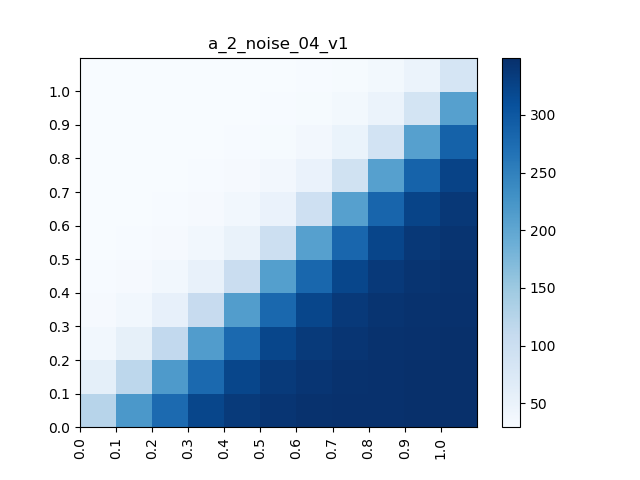
\includegraphics[width=3cm]{images/heat_maps/2_noise_04/a_2_noise_04_v1.png}}
		& \subfloat[]{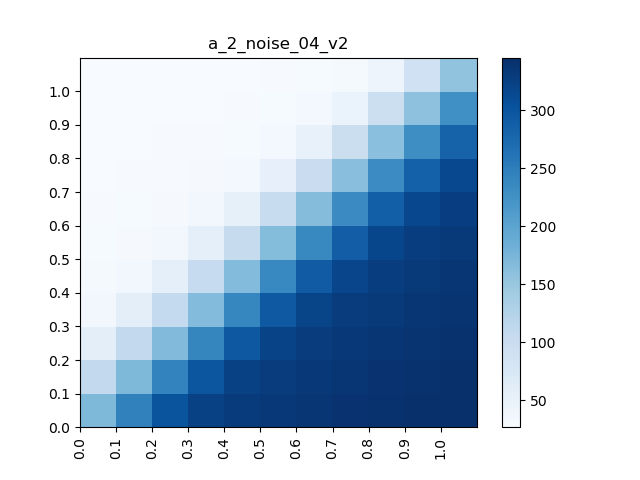
\includegraphics[width=3cm]{images/heat_maps/2_noise_04/a_2_noise_04_v2.png}} 
		&
		\subfloat[]{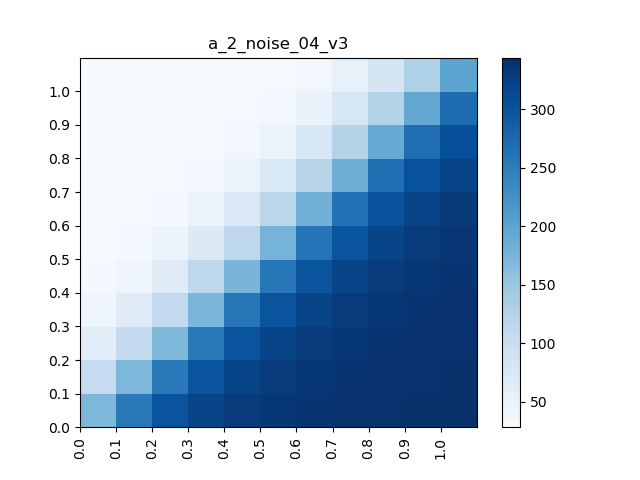
\includegraphics[width=3cm]{images/heat_maps/2_noise_04/a_2_noise_04_v3.png}}
		& \subfloat[]{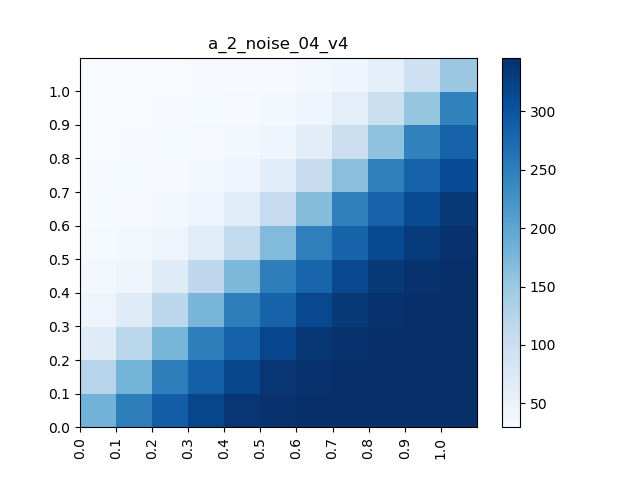
\includegraphics[width=3cm]{images/heat_maps/2_noise_04/a_2_noise_04_v4.png}} 
	\end{tabular}
	\caption{ (a) - (e) represent the distance of the classification data to a given instance of the character `a' of 5 identical instances of the same model with addition of noise and standard deviation of 0.1 that are independently trained on the same dataset. (f) - (j) show the same for standard deviation of 0.2. Every further row follows this trend and adds 0.1 more standard deviation for the training of the model.}
	\label{fig:2_noise}
\end{figure}

As can be seen in table \ref{table:2_noise} the instances confirm the theoretical prediction and get more accurate over time. They reach perfect average inverse classification accuracy of 1 for a noise addition with standard deviation of 0.3 and 0.4. In comparison to the models presented in previous chapters the standard deviation of the root mean squared error of the model with noise is also very low. This implies that a robust model can be created in one training which makes it practically useful. 

\begin{table}[!htb]
	\centering
	\caption{Results for the 2D models with the addition of noise with standard deviations of 0.1, 0.2, 0.3 and 0.4. The first five rows represent the accuracy and RMSE for each instance of the model respectively while the last two show mean and standard deviation for each respective category.}
	\begin{tabularx}{\textwidth}{ X  X  X }
		\hline
		model & accuracy & RMSE \\ 
		\hline
		2\_noise\_01\_v0 & 0.9 & 0.13\\
		2\_noise\_01\_v1 & 0.92 & 0.1 \\
		2\_noise\_01\_v2 & 0.65 & 0.42 \\
		2\_noise\_01\_v3 & 0.46 & 0.44 \\
		2\_noise\_01\_v4 & 0.41 & 0.41 \\ 
		\hline
		mean & 0.67 & 0.3 \\
		standard deviation & 0.21 & 0.15 \\
		\hline
		2\_noise\_02\_v0 & 1. &  0.08 \\
		2\_noise\_02\_v1 & 0.97 & 0.09\\
		2\_noise\_02\_v2 & 1.   & 0.02\\
		2\_noise\_02\_v3 & 0.94 & 0.16\\
		2\_noise\_02\_v4 & 1.   & 0.08\\ 
		\hline
		mean & 0.98 & 0.08 \\
		standard deviation & 0.03 & 0.04 \\
		\hline
		2\_noise\_03\_v0 & 1.   & 0.04 \\
		2\_noise\_03\_v1 & 1.   & 0.1 \\
		2\_noise\_03\_v2 & 1.   & 0.12 \\
		2\_noise\_03\_v3 & 1.   & 0.07 \\
		2\_noise\_03\_v4 & 1.   & 0.09 \\ 
		\hline
		mean & 1.0 & 0.08\\
		standard deviation & 0.0 & 0.03\\
		\hline
		2\_noise\_04\_v0 & 1. &  0.09 \\
		2\_noise\_04\_v1 & 1. &  0.1 \\
		2\_noise\_04\_v2 & 1. &  0.16 \\
		2\_noise\_04\_v3 & 1. &  0.14 \\
		2\_noise\_04\_v4 & 1. &  0.12 \\
		\hline
		mean & 1.0 & 0.12 \\
		standard deviation & 0.0 & 0.02 \\
		\hline		
	\end{tabularx}
	\label{table:2_noise}
\end{table}


\subsection{Four Dimensions}

The model was also trained with the addition of a noise layer with different standard deviations for four dimensions, i.e. four characters. Before analyzing and comparing the results the latent space is reviewed. In figures \ref{fig:4d_noise_01_a}, \ref{fig:4d_noise_02_a}, \ref{fig:4d_noise_03_a} and \ref{fig:4d_noise_04_a} the SOM of the character `a' of models with addition of noise with standard deviation 0.1, 0.2, 0.3 and 0.4 can be seen respectively. There are two major trends that come with increasing standard deviation. First, the SOMs seem to get less clustered regions representing a character. While there is a major cluster in the bottom left corner of the SOM for standard deviation of 0.1 and one at the top left of the SOM for 0.2 no regional clusters can be found for 0.3 and only vaguely for 0.4. The second trend is that borders become more fuzzy between letters while still not overlapping. In figure \ref{fig:4d_noise_01_c} and  \ref{fig:4d_noise_04_c} the SOMs for the character `c' and standard deviation of 0.1 and 0.4, respectively, can be seen. Comparing the SOMs of `a' and `c' for each model, we can see that the regions where the model with standard deviation 0.1 still has regional separation between the characters, the model with standard deviation of 0.4 has fuzzier borders but no overlap between characters. These graphics were picked for demonstration but the two analyses hold for other characters as well, even if sometimes to a lesser degree. The other characters are not depicted to save space.

\begin{figure}[!htb]
	\centering
	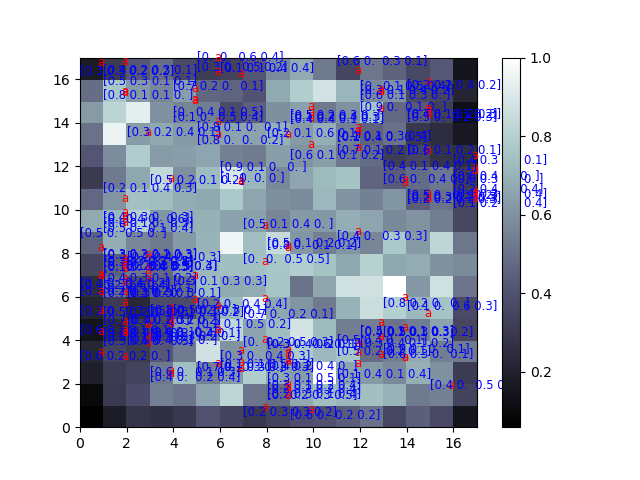
\includegraphics[width=\textwidth]{images/SOM_graphics/17x17_4d_noise_01_v0/a.png}
	\caption{SOM for version 0 of the model with the addition of noise with standard deviation of 0.1 trained on 4 characters. Only the letter `a' is represented. Red vectors are the bases for the prediction and blue characters are the result of the given prediction. The map in the background shows the average distances for each weight to their neighbors.}
	\label{fig:4d_noise_01_a}
\end{figure}

\begin{figure}[!htb]
	\centering
	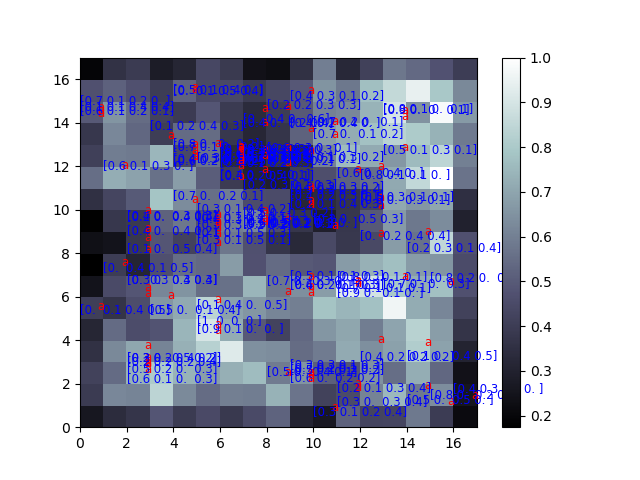
\includegraphics[width=\textwidth]{images/SOM_graphics/17x17_4d_noise_02_v0/a.png}
	\caption{SOM for version 0 of the model with the addition of noise with standard deviation of 0.2 trained on 4 characters. Only the letter `a' is represented. Red vectors are the bases for the prediction and blue characters are the result of the given prediction. The map in the background shows the average distances for each weight to their neighbors.}
	\label{fig:4d_noise_02_a}
\end{figure}

\begin{figure}[!htb]
	\centering
	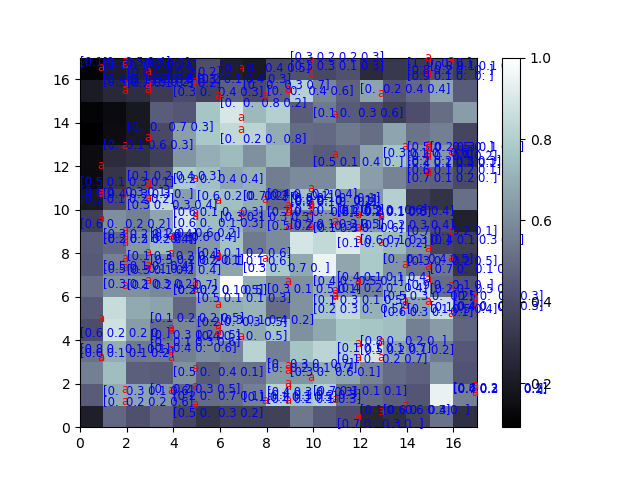
\includegraphics[width=\textwidth]{images/SOM_graphics/17x17_4d_noise_03_v0/a.png}
	\caption{SOM for version 0 of the model with with the addition of noise with standard deviation of 0.3 trained on 4 characters. Only the letter `a' is represented. Red vectors are the bases for the prediction and blue characters are the result of the given prediction. The map in the background shows the average distances for each weight to their neighbors.}
	\label{fig:4d_noise_03_a}
\end{figure}

\begin{figure}[!htb]
	\centering
	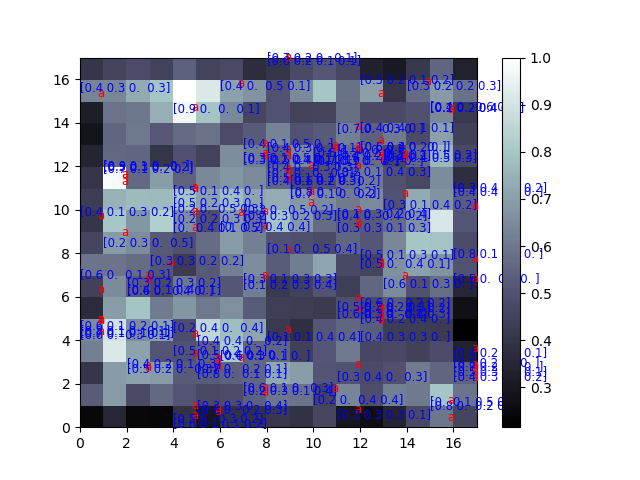
\includegraphics[width=\textwidth]{images/SOM_graphics/17x17_4d_noise_04_v0/a.png}
	\caption{SOM for version 0 of the model with with the addition of noise with standard deviation of 0.4 trained on 4 characters. Only the letter `a' is represented. Red vectors are the bases for the prediction and blue characters are the result of the given prediction. The map in the background shows the average distances for each weight to their neighbors.}
	\label{fig:4d_noise_04_a}
\end{figure}


\begin{figure}[!htb]
	\centering
	\includegraphics[width=\textwidth]{images/SOM_graphics/17x17_4d_noise_01_v0/c.png}
	\caption{SOM for version 0 of the model with the addition of noise with standard deviation of 0.1 trained on 4 characters. Only the letter `c' is represented. Red vectors are the bases for the prediction and blue characters are the result of the given prediction. The map in the background shows the average distances for each weight to their neighbors.}
	\label{fig:4d_noise_01_c}
\end{figure}


\begin{figure}[!htb]
	\centering
	\includegraphics[width=\textwidth]{images/SOM_graphics/17x17_4d_noise_04_v0/c.png}
	\caption{SOM for version 0 of the model with the addition of noise with standard deviation of 0.4 trained on 4 characters. Only the letter `c' is represented. Red vectors are the bases for the prediction and blue characters are the result of the given prediction. The map in the background shows the average distances for each weight to their neighbors.}
	\label{fig:4d_noise_04_c}
\end{figure}

After reviewing the latent spaces of the models results are analyzed and compared. In table \ref{table:4_noise} the accuracy and RMSE of every instance is depicted. Additionally the mean and standard deviation for every model can be found. The accuracy of the model gets higher and the error lower, the bigger the standard deviation of the noise layer becomes. Additionally, the standard deviation of the accuracy becomes smaller. This implies that the models with noise are very robust between different model instances making them useful for practical purposes. All models are also able to significantly beat the benchmark of the model without additions which had an accuracy of 0.49 and error of 0.35 on average. 

\begin{table}[!htb]
	\centering
	\caption{Results for the 4D models with the addition of noise with standard deviations of 0.1, 0.2, 0.3 and 0.4. The first five rows represent the accuracy and RMSE for each instance of the model respectively while the last two show mean and standard deviation for each respective category.}
	\begin{tabularx}{\textwidth}{ X  X  X }
		\hline
		model & accuracy & RMSE \\ 
		\hline
		4\_noise\_01\_v0 & 0.76 & 0.25 \\
		4\_noise\_01\_v1 & 0.94 & 0.19 \\
		4\_noise\_01\_v2 & 0.86 & 0.19 \\
		4\_noise\_01\_v3 & 0.91 & 0.21 \\
		4\_noise\_01\_v4 & 0.9  & 0.24 \\ 
		\hline
		mean & 0.88  &  0.22\\
		standard deviation & 0.06 & 0.02 \\
		\hline
		4\_noise\_02\_v0 & 0.82 & 0.26 \\
		4\_noise\_02\_v1 & 0.88 & 0.21 \\
		4\_noise\_02\_v2 & 0.94 & 0.2 \\
		4\_noise\_02\_v3 & 0.93 & 0.24 \\
		4\_noise\_02\_v4 & 0.95 & 0.17 \\ 
		\hline
		mean & 0.91 & 0.22 \\
		standard deviation & 0.05 & 0.03 \\
		\hline
		4\_noise\_03\_v0 & 0.87 & 0.2 \\
		4\_noise\_03\_v1 & 0.92 & 0.24\\
		4\_noise\_03\_v2 & 0.96 & 0.18\\
		4\_noise\_03\_v3 & 0.95 & 0.18\\
		4\_noise\_03\_v4 & 0.93 & 0.18\\
		\hline
		mean & 0.93 & 0.19 \\
		standard deviation & 0.03 & 0.02 \\
		\hline
		4\_noise\_04\_v0 & 0.89 & 0.19 \\
		4\_noise\_04\_v1 & 0.98 & 0.15\\
		4\_noise\_04\_v2 & 0.93 & 0.2\\
		4\_noise\_04\_v3 & 0.91 & 0.18\\
		4\_noise\_04\_v4 & 0.93 & 0.17\\		
		\hline
		mean & 0.93 & 0.18 \\
		standard deviation & 0.03 & 0.02 \\
		\hline 
	\end{tabularx}
	\label{table:4_noise}
\end{table}

\subsection{20 Dimensions}

\begin{table}[!htb]
	\centering
	\caption{Results for the 20D models with the addition of noise with standard deviations of 0.1, 0.2, 0.3 and 0.4. The first five rows represent the accuracy and RMSE for each instance of the model respectively while the last two show mean and standard deviation for each respective category.}
	\begin{tabularx}{\textwidth}{ X  X  X }
		\hline
		model & accuracy & RMSE \\ 
		\hline
		20\_noise\_01\_v0 & 0.37 & 0.2\\
		20\_noise\_01\_v1 & 0.34 & 0.2\\
		20\_noise\_01\_v2 & 0.37& 0.2\\
		20\_noise\_01\_v3 & 0.42& 0.19\\
		20\_noise\_01\_v4 & 0.24& 0.21\\ 
		\hline
		mean & 0.35 & 0.2\\
		standard deviation & 0.06 & 0.01 \\
		\hline
		20\_noise\_02\_v0 & 0.51 & 0.19\\
		20\_noise\_02\_v1 & 0.22 & 0.2\\
		20\_noise\_02\_v2 & 0.45 & 0.19\\
		20\_noise\_02\_v3 & 0.27 & 0.2\\
		20\_noise\_02\_v4 & 0.44 & 0.18\\ 
		\hline
		mean & 0.38 & 0.19  \\
		standard deviation & 0.11 & 0.01 \\
		\hline
		20\_noise\_03\_v0 & 0.65 & 0.17 \\
		20\_noise\_03\_v1 & 0.42 & 0.18 \\
		20\_noise\_03\_v2 & 0.33 & 0.19 \\
		20\_noise\_03\_v3 & 0.33 & 0.19 \\
		20\_noise\_03\_v4 & 0.41 & 0.18 \\
		\hline
		mean & 0.43 & 0.18 \\
		standard deviation & 0.12 & 0.01 \\
		\hline
		20\_noise\_04\_v0 & 0.33 & 0.19 \\
		20\_noise\_04\_v1 & 0.15 & 0.21\\
		20\_noise\_04\_v2 & 0.12 & 0.21\\
		20\_noise\_04\_v3 & 0.24 & 0.2\\
		20\_noise\_04\_v4 & 0.16 & 0.2\\		
		\hline
		mean & 0.2 & 0.2\\
		standard deviation & 0.08 & 0.01\\
		\hline 
	\end{tabularx}
	\label{table:20_noise}
\end{table}

The results for the noise model instances for 20D can be found in table \ref{table:20_noise}. The trends set in two and four dimensions are continued for 20, i.e. the higher the standard deviation the better the accuracy. The one big exception clearly is the addition of noise with standard deviation of 0.4. The reason for this is likely that too many adversarial examples are then in the data. When high random values are added onto the one-hot vectors the entries might be too close to each other and the network is not able to distinguish them anymore. An addition of noise with even higher standard deviation would likely result in even worse results. \\
In comparison to the model without additions there is significantly less of an increase compared to lower dimensions. Where the increase in 2D was from 0.66 to 1 and in 4D from 0.49 to 0.93, for 20D it is only from 0.35 to 0.43 average accuracy. The mean RMSE between models gets slightly better from 0.2 over 0.19 to 0.18 but absolutely these values are still very close to the random value of 0.22. This implies that the addition of noise was not able to achieve the target of making the model more confident in its predictions.\\
Interestingly, the first model for standard deviation 0.3 achieves an accuracy of 0.65 showing that even though that is not the norm, it is at least possible to get a model with better results for inverse classification than the averages.



\section{Repeller Vector}

The main problems that contribute to suboptimal results in previous sections when analyzing the latent space come from vectors that are very close to uniformly distributed. The network probably has problems identifying to which class the vector belongs if all the entries are very similar. To solve the problem a repeller vector is introduced. This simply means that $\frac{1}{n}$ uniformly distributed vectors are added to the train and test set, where $n$ is the number of classes for this training. The targets for the repeller vectors are sequences of zeros only. If the generative model is successfully repelled from forming its latent space around uniformly distributed vectors, the inverse classification might tend stronger towards one-hot vectors. 

\subsection{Two Dimensions}

As can be seen in figure \ref{fig:2_repeller} the latent space did change in comparison to a model without any additions. For all models an additional zone has been formed around the $x = y$ diagonal. The region has lower DTW distance than the other character but significantly higher than similar ones. This means that the network has learned a third, meaningless class represented through that zone and therefore achieved the aim of an repeller vector addition. Not only qualitatively, but also quantitatively the results improve, as can be seen in table \ref{table:2_repeller}. The accuracy with 0.79 on average is significantly higher compared to a naked model with 0.49 on average and the error went down in all instances resulting in 0.15 on average compared to 0.35 in the standard model. Additionally the standard deviation is very low with 0.07 for the accuracy and 0.02 for the error meaning that the model is robust between different training instances. 

\begin{figure}[!htb]
	\centering
	\begin{tabular}{ccc}
		\subfloat[]{\includegraphics[width=5cm]{images/heat_maps/2_repeller/a_2_repeller_v0.png}} 
		& \subfloat[]{\includegraphics[width=5cm]{images/heat_maps/2_repeller/a_2_repeller_v1.png}}
		& \subfloat[]{\includegraphics[width=5cm]{images/heat_maps/2_repeller/a_2_repeller_v2.png}} \\
		\subfloat[]{\includegraphics[width=5cm]{images/heat_maps/2_repeller/a_2_repeller_v3.png}}
		& \subfloat[]{\includegraphics[width=5cm]{images/heat_maps/2_repeller/a_2_repeller_v4.png}} 
		& \subfloat[]{\includegraphics[width=5cm]{images/heat_maps/2_repeller/b_2_repeller_v0.png}}
	\end{tabular}
	\caption{ (a) - (e) represent the distance of the classification data to a given instance of the character `a' of five instances of the 2D models with repeller addition that are independently trained on the same dataset. (f) shows the distance of the same model as depicted in (a) to the character `b'. }
	\label{fig:2_repeller}
\end{figure}


\begin{table}[!htb]
	\centering
	\caption{Results for the 2D models with the addition of repeller vectors. The first five rows represent the accuracy and RMSE for each instance of the model respectively while the last two show mean and standard deviation for each respective category.}
	\begin{tabularx}{\textwidth}{ X  X  X }
		\hline
		model & accuracy & RMSE \\ 
		\hline
		2\_repeller\_v0 & 0.88 & 0.12 \\
		2\_repeller\_v0 & 0.69 & 0.15 \\
		2\_repeller\_v0 & 0.72 & 0.18 \\
		2\_repeller\_v0 & 0.84 & 0.15 \\
		2\_repeller\_v0 & 0.83 & 0.15 \\
		\hline 
		mean & 0.79 & 0.15 \\
		standard deviation & 0.07 & 0.02 \\
		\hline
	\end{tabularx}
	\label{table:2_repeller}
\end{table}


\subsection{Four Dimensions}

To analyze the latent space of the repeller models with four dimensions a class needs to be shown that is not even mentioned for all other sections. While labeling the sequences that are produced by the generative models, there are some which are unrecognizable. These are labeled with an `x'. For all other models so far only very few instances have been put in that class and mostly it was just when the model generated a mixture between two characters when two entries in the vector were around the same value. In the case of the repeller model much more sequences needed to be labeled with `x' since the sequences were just entirely unrecognizable. In figure \ref{fig:4d_repeller_x} all the values of the `x' class can be seen. Notably, most of the vectors producing unrecognizable results, and therefore being labeled with `x', are very close to uniformly distributed, i.e. having very similar values for all entries. This is not really surprising given that the model was trained to generate sequences of zeros when presented with exactly uniformly distributed vectors. In the inverse, all characters that do have labels, have very high values in their respective entries. An example of this can be found in figure \ref{fig:4d_repeller_d}, where the SOM for the character `d' is shown. Most vectors have values of 0.5 or higher at the 4th entry, which stands for the class of character `d'. \\

\begin{figure}[!htb]
	\centering
	\includegraphics[width=\textwidth]{images/SOM_graphics/17x17_4d_repeller_v0/x.png}
	\caption{SOM for version 0 of the repeller model trained on 4 characters. Only the class `x' is shown which stands for unrecognizable characters. Red vectors are the bases for the prediction and blue characters are the result of the given prediction. The map in the background shows the average distances for each weight to their neighbors.}
	\label{fig:4d_repeller_x}
\end{figure}

\begin{figure}[!htb]
	\centering
	\includegraphics[width=\textwidth]{images/SOM_graphics/17x17_4d_repeller_v0/d.png}
	\caption{SOM for version 0 of the repeller model trained on 4 characters. Only the letter `d' is represented. Red vectors are the bases for the prediction and blue characters are the result of the given prediction. The map in the background shows the average distances for each weight to their neighbors.}
	\label{fig:4d_repeller_d}
\end{figure}

The qualitative evaluation of the repeller models can be found in table \ref{table:4_repeller}. The accuracy of the model is 0.58 on average beating the accuracy of the model without additions of 0.49. The error of 0.27 on average is also lower than the 0.35 of the standard model. The standard deviation between different instances of the model trained on the same data is rather low with 0.11 for accuracy and only 0.05 for the RMSE. This implies a robust model but also that a classification of around 0.69, like in model instance 2, is very likely close to the upper bound for classification with this technique. 

\begin{table}[!htb]
	\centering
	\caption{Results for the 4D models with the addition of repeller vectors. The first five rows represent the accuracy and RMSE for each instance of the model respectively while the last two show mean and standard deviation for each respective category.}
	\begin{tabularx}{\textwidth}{ X  X  X }
		\hline
		model & accuracy & RMSE \\ 
		\hline
		4\_repeller\_v0 & 0.59 & 0.29 \\ 
		4\_repeller\_v1 & 0.65 & 0.26 \\
		4\_repeller\_v2 & 0.69 & 0.21 \\ 
		4\_repeller\_v3 & 0.37 & 0.36 \\ 
		4\_repeller\_v4 & 0.61 & 0.24 \\
		\hline
		mean & 0.58 & 0.27\\
		standard deviation & 0.11 & 0.05 \\
		\hline
	\end{tabularx}
	\label{table:4_repeller}
\end{table}

\subsection{20 Dimensions}


\begin{table}[!htb]
	\centering
	\caption{Results for the 20D models with the addition of repeller vectors. The first five rows represent the accuracy and RMSE for instance of the each model respectively while the last two show mean and standard deviation for each respective category.}
	\begin{tabularx}{\textwidth}{ X  X  X }
		\hline
		model & accuracy & RMSE \\ 
		\hline
		20\_repeller\_v0 & 0.21 & 0.2 \\ 
		20\_repeller\_v1 & 0.34 & 0.2 \\
		20\_repeller\_v2 & 0.26 & 0.2 \\ 
		20\_repeller\_v3 & 0.33 & 0.19 \\ 
		20\_repeller\_v4 & 0.33 & 0.2 \\
		\hline
		mean & 0.29 & 0.2\\
		standard deviation & 0.05 & 0.0 \\
		\hline
	\end{tabularx}
	\label{table:20_repeller}
\end{table}

As can be seen in table \ref{table:20_repeller} the addition of repeller vectors is no improvement to a model with no additions. A classification rate of 0.29 on average is worse than the 0.35 given by the naked model. The mean RMSE of 0.2 is exactly the same as in the other model.\\
In conclusion, the addition of repeller vectors seems to increase the performance of the 2D and 4D model but fails to reproduce that result for 20D.

\section{Addition of Types}

For the following chapter two main problems are tackled. Since the inverse classification process consistently converged against none one-hot vectors for some character sequences it seems likely to assume that the model might have learned different types of a character, i.e. an 'a' with a big belly and a small belly. The second problem is the number of samples that need to be trained. As described in the introduction, a main purpose of inverse classification is to downscale the number of training data to a minimum. \\
Therefore a k-means clustering algorithm is used to generate four clusters or types for every character in the dataset. The center of every cluster is taken as a representative for each type. The types are stored in two dimensional one-hot vectors, i.e. in a 2D model $[[1,0,0,0], [0,0,0,0]]$ would represent the first type of the character 'a'. \\
The inverse classification in this section is done on reduced types, i.e. the a sum is applied over the type dimension to make the model comparable with the standard approach. If, for example, the inverse classification resulted in $[[0.25,0.25,0.25,0],[0.25,0,0,0]]$, the resulting reduced vector would be $[0.75,0.25]$. 

\subsection{Two Dimensions}

\begin{table}[!htb]
	\centering
	\caption{Results for the 2D models trained on typed data. The first five rows represent the accuracy and RMSE for each instance of the model while the last two show mean and standard deviation for each respective category.}
	\begin{tabularx}{\textwidth}{ X  X  X }
		\hline
		model & accuracy & RMSE \\ 
		\hline
		2\_types\_v0 & 0.57 & 0.47 \\ 
		2\_types\_v1 & 0.6 & 0.45 \\
		2\_types\_v2 & 0.94 & 0.15 \\ 
		2\_types\_v3 & 1.  & 0.28 \\ 
		2\_types\_v4 & 0.84 & 0.33 \\ \hline
		mean & 0.79 &  0.34\\
		standard deviation & 0.17 & 0.12\\
		\hline
	\end{tabularx}
	\label{table:2_types}
\end{table}

Results for the 2D models of the implementation with types can be found in table \ref{table:2_types}. There are two primary findings that can be seen in the five trained instances. First, the deviation between instances is really high given that the accuracies range from 0.57 to 1. Second, the mean RMSE is really high, even when the model has perfect accuracy. There could be multiple competing explanations for that: a) the model learned very accurate representations of the different types of characters and therefore represents a previously unseen 'a' as a mixture between types of 'a' and 'b' or b) the model just was not able to grasp the differences between types and therefore is unsure about its prediction. Looking at results from previous chapters and for typed data at four and 20 dimensions hypotheses b) seems more likely, since accuracies become lower quickly.

\subsection{Four Dimensions}

\begin{table}[!htb]
	\centering
	\caption{Results for the 4D models trained on typed data. The first five rows represent the accuracy and RMSE for each instance of the model while the last two show mean and standard deviation for each respective category.}
	\begin{tabularx}{\textwidth}{ X  X  X }
		\hline
		model & accuracy & RMSE \\ 
		\hline
		4\_types\_v0 & 0.18 &0.45 \\ 
		4\_types\_v1 & 0.24 &0.43 \\
		4\_types\_v2 & 0.37 &0.43 \\ 
		4\_types\_v3 & 0.2  &0.47 \\ 
		4\_types\_v4 & 0.34 &0.42 \\ \hline
		mean & 0.27 &  0.44\\
		standard deviation & 0.08 & 0.02\\
		\hline
	\end{tabularx}
	\label{table:4_types}
\end{table}

Results for the 4D implementation of the typed experiment can be seen in table \ref{table:4_types}. With a mean of 0.27 for accuracy and 0.44 for the RMSE the results of this experiment are very close to the guessing values of 0.25 and 0.43 respectively. Therefore it seems likely that the addition of types does not make a distinction within characters or between classes more clearly but rather adds an additional degree of complexity that the model cannot handle. 

\subsection{20 Dimensions}

\begin{table}[!htb]
	\centering
	\caption{Results for the 20D models trained on typed data. The first five rows represent the accuracy and RMSE for each instance of the model while the last two show mean and standard deviation for each respective category.}
	\begin{tabularx}{\textwidth}{ X  X  X }
		\hline
		model & accuracy & RMSE \\ 
		\hline
		20\_types\_v0 & 0.07 & 0.22 \\ 
		20\_types\_v1 & 0.08 & 0.22 \\
		20\_types\_v2 & 0.14 & 0.22 \\ 
		20\_types\_v3 & 0.05 & 0.22 \\ 
		20\_types\_v4 & 0.09 & 0.22 \\ \hline
		mean & 0.08 &  0.22\\
		standard deviation & 0.03 & 0.0\\
		\hline
	\end{tabularx}
	\label{table:20_types}
\end{table}

For 20 characters the trend that was already seen for four continues. As table \ref{table:20_types} shows, the mean accuracy of 0.08 and mean RMSE of 0.22 do not significantly diverge from random guessing of 0.05 and 0.22. It therefore seems plausible to conclude that the addition of types is not an information gain that the model handles very well. 

\section{Addition of Types with Noise}

To test if the addition of types is necessarily counterproductive, we add noise to it, since that was so far the most successful addition from previous experiments. \\
The setup of the model and inverse classification procedure are done exactly as in the previous section but noise is added. The noise is drawn from a Gaussian distribution with mean 0 and different standard deviations. The resulting vector is clipped such that its values stay between 0 and 1. The standard deviations chosen are the best results from previous experiments for each dimensionality respectively, i.e. 0.4 for 2D, 0.4 for 4D and 0.3 for 20D.

\subsection{Two Dimensions}

\begin{table}[!htb]
	\centering
	\caption{Results for the 2D models with the addition of noise with standard deviation 0.4 trained on typed data. The first five rows represent the accuracy and RMSE for each instance of the model while the last two show mean and standard deviation for each respective category.}
	\begin{tabularx}{\textwidth}{ X  X  X }
		\hline
		model & accuracy & RMSE \\ 
		\hline
		2\_types\_noise\_04\_v0 & 1.  & 0.18 \\ 
		2\_types\_noise\_04\_v1 & 0.94& 0.29 \\
		2\_types\_noise\_04\_v2 & 0.95& 0.25 \\ 
		2\_types\_noise\_04\_v3 & 0.4 & 0.54 \\ 
		2\_types\_noise\_04\_v4 & 0.98& 0.33 \\ \hline
		mean & 0.85 &  0.32\\
		standard deviation & 0.23 & 0.12\\
		\hline
	\end{tabularx}
	\label{table:2_types_noise_04}
\end{table}

As can be seen in table \ref{table:2_types_noise_04} the addition of noise does increase the accuracy and decrease the variance between models. Even though the mean accuracy only changes from 0.79 to 0.85 and the mean RMSE from 0.34 to 0.32 the mean values might be a bit deceiving since they are primarily pulled down by model version 3, a big outlier. However, the existence of that outlier only shows that even with added noise the addition of types method is not robust and therefore, in this implementation, not useful for practical purposes.

\subsection{Four Dimensions}


\begin{table}[!htb]
	\centering
	\caption{Results for the 4D models with the addition of noise with standard deviation 0.4 trained on typed data. The first five rows represent the accuracy and RMSE for each model instance of the while the last two show mean and standard deviation for each respective category.}
	\begin{tabularx}{\textwidth}{ X  X  X }
		\hline
		model & accuracy & RMSE \\ 
		\hline
		4\_types\_noise\_04\_v0 & 0.9  &0.37 \\ 
		4\_types\_noise\_04\_v1 & 0.88 &0.35 \\
		4\_types\_noise\_04\_v2 & 0.86 &0.31 \\ 
		4\_types\_noise\_04\_v3 & 0.72 &0.36 \\ 
		4\_types\_noise\_04\_v4 & 0.61 &0.37 \\ \hline
		mean & 0.79 &  0.35\\
		standard deviation & 0.11 & 0.02\\
		\hline
	\end{tabularx}
	\label{table:4_types_noise_04}
\end{table}

The results for the addition of noise on typed data for 4 characters can be found in table \ref{table:4_types_noise_04}. With a mean accuracy of 0.79 and a mean RMSE of 0.35 we can see that the accuracy gets significantly better compared to the type model without noise but the confidence of the model in its prediction stays rather low since 0.35 is not too far from 0.43. 

\subsection{20 Dimensions}

\begin{table}[!htb]
	\centering
	\caption{Results for the 20D models with the addition of noise with standard deviation 0.3 trained on typed data. The first five rows represent the accuracy and RMSE for each instance of the model while the last two show mean and standard deviation for each respective category.}
	\begin{tabularx}{\textwidth}{ X  X  X }
		\hline
		model & accuracy & RMSE \\ 
		\hline
		20\_types\_noise\_04\_v0 & 0.17 &0.21 \\ 
		20\_types\_noise\_04\_v1 & 0.06 &0.22 \\
		20\_types\_noise\_04\_v2 & 0.08 &0.22 \\ 
		20\_types\_noise\_04\_v3 & 0.06 &0.22 \\ 
		20\_types\_noise\_04\_v4 & 0.09 &0.22 \\ \hline
		mean & 0.09 &  0.22\\
		standard deviation & 0.04 & 0.0\\
		\hline
	\end{tabularx}
	\label{table:20_types_noise_03}
\end{table}

Even though the addition of noise was able to increase the accuracy for two and four characters it seems like that trend is not continued with 20. As represented in table \ref{table:20_types_noise_03} a mean accuracy of 0.09 and a mean RMSE of 0.22 are very close to the random guessing values 0.05 and 0.22 respectively. This result seems to imply that the addition of types to the data does not increase the predictive value of the inverse classification, even when noise is added.

\section{Sparse Data with Noise}

Since the results of the addition of noise on the typed data in the previous section resulted in high accuracy but still high error rates, in this section the types are flattened but the sparse data is kept. This means that what has been an `a' of type 0 in the last section in 2D, i.e. $[[1,0,0,0],[0,0,0,0]]$ now just becomes $[1,0]$. This implies that every class of characters still has only four instances and is therefore called sparse data. These four instances, however, are the cluster means from the k-means clustering and therefore should contain more information than four randomly chosen characters. \\
The noise is drawn from a Gaussian distribution with mean 0 and different standard deviations. The resulting vector is clipped such that its values stay between 0 and 1. The standard deviations chosen are the best results from previous experiments for each dimensionality respectively, i.e. 0.4 for 2D, 0.4 for 4D and 0.3 for 20D.


\subsection{Two Dimensions}

\begin{table}[!htb]
	\centering
	\caption{Results for the 2D models with the addition of noise with standard deviation 0.4 trained on sparse data. The first five rows represent the accuracy and RMSE for each instance of the model while the last two show mean and standard deviation for each respective category.}
	\begin{tabularx}{\textwidth}{ X  X  X }
		\hline
		model & accuracy & RMSE \\ 
		\hline
		2\_sparse\_noise\_04\_v0 & 1. &  0.16 \\ 
		2\_sparse\_noise\_04\_v1 & 0.94 & 0.11 \\
		2\_sparse\_noise\_04\_v2 & 1.  & 0.09 \\ 
		2\_sparse\_noise\_04\_v3 & 1.  & 0.15 \\ 
		2\_sparse\_noise\_04\_v4 & 0.94 & 0.14 \\ \hline
		mean & 0.97 & 0.13\\
		standard deviation & 0.03 & 0.03\\
		\hline
	\end{tabularx}
	\label{table:2_sparse_noise_04}
\end{table}

As shown in table \ref{table:2_sparse_noise_04} the mean accuracy of 0.97  is very high and the mean RMSE of 0.13 very low given that the network is trained on only four representations of each character. In comparison to the values 1.0 and 0.13 that the same network achieves on multiple hundreds of samples per character we can see that removing lots of training data does not have a major impact on the ability of the generative model to learn the concepts, at least for 2D.

\subsection{Four Dimensions}

\begin{table}[!htb]
	\centering
	\caption{Results for the 4D models with the addition of noise with standard deviation 0.4 trained on sparse data. The first five rows represent the accuracy and RMSE for each instance of the model while the last two show mean and standard deviation for each respective category.}
	\begin{tabularx}{\textwidth}{ X  X  X }
		\hline
		model & accuracy & RMSE \\ 
		\hline
		2\_sparse\_noise\_04\_v0 & 0.98 & 0.17 \\ 
		2\_sparse\_noise\_04\_v1 & 0.96 & 0.2  \\
		2\_sparse\_noise\_04\_v2 & 0.93 & 0.17\\ 
		2\_sparse\_noise\_04\_v3 & 0.95 & 0.17\\ 
		2\_sparse\_noise\_04\_v4 & 1.  & 0.17 \\ \hline
		mean & 0.97 & 0.18\\
		standard deviation & 0.02 & 0.01\\
		\hline
	\end{tabularx}
	\label{table:4_sparse_noise_04}
\end{table}

The trend that was set by sparse data for two characters continues for four. As depicted in table \ref{table:4_sparse_noise_04} the mean classification accuracy of 0.97 is even bigger than the 0.93 that were achieved by the model trained on all data. This, however, is likely due to statistical fluctuation, i.e. the sparse models being over average good or the others under average bad, since there is no good reason for a model learning a concept better when only training on a subset of the data. The mean RMSE is exactly the same, both for normal and sparse data. Additionally, the standard deviation of both accuracy and RSME is very low, implying that the model performance is very robust over multiple training sessions.

\subsection{20 Dimensions}  

\begin{table}[!htb]
	\centering
	\caption{Results for the 20D models with the addition of noise with standard deviation 0.3 trained on sparse data. The first five rows represent the accuracy and RMSE for each instance of the model while the last two show mean and standard deviation for each respective category.}
	\begin{tabularx}{\textwidth}{ X  X  X }
		\hline
		model & accuracy & RMSE \\ 
		\hline
		20\_sparse\_noise\_03\_v0 & 0.47 & 0.18\\ 
		20\_sparse\_noise\_03\_v1 & 0.39 & 0.2 \\
		20\_sparse\_noise\_03\_v2 & 0.49 & 0.18 \\ 
		20\_sparse\_noise\_03\_v3 & 0.5  & 0.19 \\ 
		20\_sparse\_noise\_03\_v4 & 0.58 & 0.18 \\ \hline
		mean & 0.49 & 0.19\\
		standard deviation & 0.06 & 0.01\\
		\hline
	\end{tabularx}
	\label{table:20_sparse_noise_03}
\end{table}

The results for the 20D model trained on sparse data with the addition of noise with standard deviation of 0.3 can be seen in table \ref{table:20_sparse_noise_03}. The model outperforms all other previously tested inverse classification models with an average accuracy of 0.49. This result is surprising, since it is trained on a subset of the data on which the noise\_20\_03 models were trained. The results might be due to statistical fluctuations.

\section{Comparison with Standard Classification}

To evaluate the classification quality of the model the results are compared to a standard classification approach. This comparison model is constructed in a way that resembles the models for inverse classification as much as possible. The network uses LSTMs with one hidden layer of size 205 combined sequentially with a fully connected layer (FC). The number of units for the FC are the number of classes it is trained on. The activation function for the last layer is the softmax function (softmax$(x) = \frac{\exp(x_i)}{\sum_j \exp(x_j)}$), since the output then consists of values between 0 and 1 representing the likelihood of a class being the correct one. 
For the training the Adam optimizer (\cite{AdamKingmaB14}) is used.
Since the inverse classification was done with a mean squared error (MSE), the comparison model set of five model instances is also trained on MSE to make it as comparable as possible.\\
It is trained on the same data and trains for the same number of epochs as all other models have been trained on. To test for robustness five isntances with the same specifications are trained. The results are measured in the same way as all other models before, i.e. the accuracy and the RMSE of the result. \\
To compare the standard approach to the sparse data experiments conducted in the last three sections, additional instances of models are trained on the same data as the typed and sparse data models. For the comparison with types, the standard approach is not trained on typed data, but just on sparse data. This is the case because the types are merely thought to enhance the process of generation, thereby creating better representations, not influencing the classification process itself. 

\subsection{Two Dimensions}


\begin{table}[!htb]
	\centering
	\caption{Results for the 2D models with a standard sequence classification approach. The first five rows represent the accuracy and RMSE for each instance of the model while the last two show mean and standard deviation for each respective category.}
	\begin{tabularx}{\textwidth}{ X  X  X }
		\hline
		model & accuracy & RMSE \\ 
		\hline
		2\_comparison\_v0 & 1.0 & 0.0 \\ 
		2\_comparison\_v1 & 1.0 & 0.0 \\
		2\_comparison\_v2 & 1.0 & 0.0 \\ 
		2\_comparison\_v3 & 1.0 & 0.0 \\ 
		2\_comparison\_v4 & 1.0 & 0.0  \\ \hline
		mean & 1.0 & 0.0\\
		standard deviation & 0.0 & 0.0 \\
		\hline
	\end{tabularx}
	\label{table:2_comparison_mse}
\end{table}



\begin{table}[!htb]
	\centering
	\caption{Results for the 2D models with a standard sequence classification approach trained on sparse data. The first five rows represent the accuracy and RMSE for each instance of the model while the last two show mean and standard deviation for each respective category.}
	\begin{tabularx}{\textwidth}{ X  X  X }
		\hline
		model & accuracy & RMSE \\ 
		\hline
		2\_comparison\_sparse\_v0 & 1.   & 0.  \\ 
		2\_comparison\_sparse\_v1 & 0.97 & 0.18 \\
		2\_comparison\_sparse\_v2 & 0.97 & 0.18 \\ 
		2\_comparison\_sparse\_v3 & 0.95 & 0.22 \\ 
		2\_comparison\_sparse\_v4 & 1.   & 0.   \\ \hline
		mean & 0.98 & 0.11\\
		standard deviation & 0.02 & 0.09\\
		\hline
	\end{tabularx}
	\label{table:2_comparison_sparse}
\end{table}

As can be seen in table \ref{table:2_comparison_mse} when trained on many data points per individual class the comparison model is able to reach an accuracy of 1 and a RMSE of 0. This shows not only that it is able to identify each single class, but also that its confidence for the prediction is maximal. \\
In comparison when trained on sparse data, as can be found in table \ref{table:2_comparison_sparse}, the accuracy for some models is 1 but some are not able to learn all categories correctly. The high RMSE of the imperfect models is likely due to the high confidence in the inaccurate prediction. These results show, however, that even a model trained on only four examples per class can reach perfect results. 

\subsection{Four Dimensions}

\begin{table}[!htb]
	\centering
	\caption{Results for the 4D models with a standard sequence classification approach. The first five rows represent the accuracy and RMSE for each instance of the model while the last two show mean and standard deviation for each respective category.}
	\begin{tabularx}{\textwidth}{ X  X  X }
		\hline
		model & accuracy & RMSE \\ 
		\hline
		4\_comparison\_v0 & 0.93 & 0.16\\ 
		4\_comparison\_v1 & 0.95 & 0.12 \\
		4\_comparison\_v2 & 0.92 & 0.16 \\ 
		4\_comparison\_v3 & 0.95 & 0.12 \\ 
		4\_comparison\_v4 & 0.96 & 0.1  \\ \hline
		mean & 0.94 & 0.13\\
		standard deviation & 0.02 & 0.03\\
		\hline
	\end{tabularx}
	\label{table:4_comparison_mse}
\end{table}


\begin{table}[!htb]
	\centering
	\caption{Results for the 4D models with a standard sequence classification approach trained on sparse data. The first five rows represent the accuracy and RMSE for each instance of the model while the last two show mean and standard deviation for each respective category.}
	\begin{tabularx}{\textwidth}{ X  X  X }
		\hline
		model & accuracy & RMSE \\ 
		\hline
		4\_comparison\_sparse\_v0 & 0.95 & 0.16\\ 
		4\_comparison\_sparse\_v1 & 0.91 & 0.21 \\
		4\_comparison\_sparse\_v2 & 0.93 & 0.18 \\ 
		4\_comparison\_sparse\_v3 & 0.94 & 0.17 \\ 
		4\_comparison\_sparse\_v4 & 0.97 & 0.13 \\ \hline
		mean & 0.94 & 0.17\\
		standard deviation & 0.02 & 0.03\\
		\hline
	\end{tabularx}
	\label{table:4_comparison_sparse}
\end{table}

Depicted in table \ref{table:4_comparison_mse} and \ref{table:4_comparison_sparse} the results for the comparison models trained on the entirety of the data and sparse data are depicted. Interestingly, the quality of the prediction is very similar despite the significantly lesser amount of data for the sparse model. The only small difference is in the RMSE of the models, where the sparse is slightly higher with an average 0.17 compared to an average of 0.13 for the other model. Besides a slight advantage on being more confident in the correct predictions, there does not seem to be an advantage in training on many different examples. 

\subsection{20 Dimensions}


\begin{table}[!htb]
	\centering
	\caption{Results for the 20D models with a standard sequence classification approach. The first five rows represent the accuracy and RMSE for each instance of the model while the last two show mean and standard deviation for each respective category.}
	\begin{tabularx}{\textwidth}{ X  X  X }
		\hline
		model & accuracy & RMSE \\ 
		\hline
		20\_comparison\_v0 & 0.98 & 0.04\\ 
		20\_comparison\_v1 & 0.97 & 0.04 \\
		20\_comparison\_v2 & 0.95 & 0.06 \\ 
		20\_comparison\_v3 & 0.97 & 0.05 \\ 
		20\_comparison\_v4 & 0.96 & 0.05 \\ \hline
		mean & 0.97 & 0.05\\
		standard deviation & 0.01 & 0.01\\
		\hline
	\end{tabularx}
	\label{table:20_comparison_mse}
\end{table}


\begin{table}[!htb]
	\centering
	\caption{Results for the 20D models with a standard sequence classification approach trained on sparse data. The first five rows represent the accuracy and RMSE for each instance of the model while the last two show mean and standard deviation for each respective category.}
	\begin{tabularx}{\textwidth}{ X  X  X }
		\hline
		model & accuracy & RMSE \\ 
		\hline
		20\_comparison\_sparse\_v0 & 0.76 & 0.15\\ 
		20\_comparison\_sparse\_v1 & 0.63 & 0.16 \\
		20\_comparison\_sparse\_v2 & 0.6  & 0.17 \\ 
		20\_comparison\_sparse\_v3 & 0.38 & 0.19 \\ 
		20\_comparison\_sparse\_v4 & 0.68 & 0.15 \\ \hline
		mean & 0.61 & 0.17\\
		standard deviation & 0.13 & 0.02\\
		\hline
	\end{tabularx}
	\label{table:20_comparison_sparse}
\end{table}

The comparison results for the 20D models can be found in table \ref{table:20_comparison_mse} for normal training procedure. For the standard approach, the results are quite good. On average correctly classifying 0.97 of the test data with an average RMSE of only 0.05 without any major outliers.\\
Interestingly, the average accuracy and RMSE are even better than the same procedure for only four characters, reviewed in the previous subsection. This might be caused by the characters `a', `b', `c' and `d' having a higher average complexity then the rest and therefore being harder to learn. This, however, is only speculation and no further research was conducted regarding that question. \\
The results for training on sparse data can be found in table \ref{table:20_comparison_sparse}. The models average accuracy is 0.61, being pulled down by the outlier of model version 3. The RMSE of all models is rather high with 0.17 on average which is only 0.05 smaller than the RMSE of a random guess. This likely implies that the confidence of the models in their predictions was not very high, i.e. it did not converge towards a one-hot vector. \\
It is also significantly worse than the comparison models that were not trained on sparse data, implying that either a) some characters in the other 16 classes are hard to capture in only four samples per class or b) that a higher number of classes also demands more training samples per class in a nonlinear fashion. 



% Main chapter 5:
% Conclusion 

\chapter{Conclusion}
\label{chap:Conclusion}

To conclude the work, the strengths and weaknesses of the models compared to randomness and to a standard classification approach are discussed and future research is outlined. 

\section{Quality of the Model}

To evaluate the quality of the model two questions need to be answered. 1. Does it work at all, i.e. is it better than randomness? And if that is the case: 2. Is it better than other approaches with similar infrastructure, i.e. the same number of parameters and the same kinds of artificial neural networks used?\\
In table \ref{table:comparison_all} the average accuracy and the average RMSE for all different techniques and dimensions discussed in this paper can be found. 

\begin{table}[!htb]
	\centering
	\caption{Every model tested in the work with respective accuracy, root mean squared error (RMSE), standard deviation of accuracy and error and values for random guessing.}
	\begin{tabularx}{\textwidth}{p{5cm} X X X X}
		\hline
		model & accuracy & RMSE & std acc. & std RMSE\\ 
		\hline
		naked\_2 & 0.66 & 0.38 & 0.17 & 0.14 \\
		ds\_2 & 0.54 & 0.49 & 0.12 & 0.09 \\
		noise\_01\_2 & 0.67 & 0.3 & 0.21 & 0.15 \\
		noise\_02\_2 & 0.98 & 0.08 & 0.03 & 0.04 \\
		noise\_03\_2 & 1.0 & 0.08 & 0 & 0.03 \\
		noise\_04\_2 & 1.0 & 0.12 & 0 & 0.02 \\
		repeller\_2 & 0.79 & 0.15 & 0.07 & 0.02 \\
		types\_2 & 0.79 & 0.34 & 0.17 & 0.12 \\
		types\_noise\_04\_2 & 0.85 & 0.32 & 0.23 & 0.12 \\
		sparse\_noise\_04\_2 & 0.97 & 0.13 & 0.03 & 0.03 \\
		comparison\_mse\_2 & 1.0 &0.0& 0.0& 0.0 \\
		comparison\_sparse\_2 & 0.98 & 0.11 & 0.02 & 0.09 \\
		random\_values & 0.5 & 0.5 & - & - \\
		\hline
		naked\_4 & 0.49 & 0.38 & 0.14 & 0.05 \\
		ds\_4 & 0.65 & 0.3 & 0.23 & 0.09 \\
		noise\_01\_4 & 0.88 & 0.22 & 0.06 & 0.02 \\
		noise\_02\_4 & 0.91 & 0.22 & 0.05 & 0.03 \\
		noise\_03\_4 & 0.93 & 0.19 & 0.03 & 0.02 \\
		noise\_04\_4 & 0.93 & 0.18 & 0.03& 0.02 \\
		repeller\_4 & 0.58 & 0.27 & 0.11 & 0.05 \\
		types\_4 & 0.27 & 0.44 & 0.08 & 0.02 \\
		types\_noise\_04\_4 & 0.79 & 0.35 & 0.11 & 0.02 \\
		sparse\_noise\_04\_4 & 0.97 & 0.18 & 0.02 & 0.01 \\
		comparison\_mse\_4 & 0.94 & 0.13& 0.02& 0.03 \\
		comparison\_sparse\_4 & 0.94& 0.17 & 0.02& 0.03 \\		
		random\_values & 0.25 & 0.43 & - & - \\
		\hline
		naked\_20 & 0.35 & 0.2 & 0.05 & 0.0 \\
		ds\_20 & 0.32 & 0.2 & 0.09 & 0.01 \\
		noise\_01\_20 & 0.35 & 0.2 & 0.06 & 0.01 \\
		noise\_02\_20 & 0.38 & 0.19 & 0.11 & 0.01 \\
		noise\_03\_20 & 0.43 & 0.18 & 0.12 & 0.01 \\
		noise\_04\_20 & 0.2 & 0.2 & 0.08 & 0.01 \\
		repeller\_20 & 0.29 & 0.2 & 0.05 & 0.0 \\
		types\_20 & 0.08 & 0.22 & 0.03 & 0.0 \\
		types\_noise\_03\_20 & 0.09 & 0.22 & 0.04 & 0.0 \\
		sparse\_noise\_03\_20 & 0.49 & 0.19 & 0.06 & 0.01 \\
		comparison\_mse\_20 & 0.97 & 0.05 & 0.01& 0.01 \\
		comparison\_sparse\_20 & 0.61 & 0.17& 0.13 & 0.02 \\
		random\_values & 0.05 & 0.22 & - & - \\
		\hline
	\end{tabularx}
	\label{table:comparison_all}
\end{table}

\section{Interpretation}

Quantitatively, multiple results can be seen throughout the experiments. \\
a) Double stacking LSTMs does not increase performance.\\
b) Addition of noise improves the conceptual representation within latent space increasing accuracy of the models. However, there seems to be a point at which further addition of noise is more confusing than helpful which can be especially seen for the 20D model. \\
c) The addition of an additional class of repeller vectors does not seem to have a strong effect. While increasing accuracy for the 2D models the improvement vanishes with more dimensions. \\
d) The addition of types adds an additional degree of complexity to the process that higher dimensional models, i.e. 4D and 20D, cannot handle anymore and is therefore harmful. \\
e) The addition of noise on types is able to improve results for lower dimension but unable to repair the problems of 20D typed representations. \\
f) The removal of many data points to generate sparse data does close to no harm at all. In the case of 4D and 20D it even outperforms the models trained on all data slightly for unclear reasons. \\
g) The comparison models show mostly similar or better classification qualities compared to the best other models. Especially for 20D the difference is very significant. \\
h) When the comparison model is trained on sparse data the classification quality stays similar for 2D and 4D but drops very much for 20D. \\
i) RMSE correlates strongly with the classification accuracy, the quality of internal representations therefore affect correctness of and confidence in the model in the same way. \\
j) On average, all models outperform random guessing, even if individual instances are worse for 20 dimensions. \\

Qualitatively, the most important result, which also holds true for all experiments, is that the quality of the inverse classification model is very much determined by the quality of the internal representations of the generative model, i.e. the latent space. This can be found throughout all heat maps, where a clear separation along the $x=y$ axis implies better results for the inverse classification. It can also be seen within the SOMs where the separation of clusters within the latent space implies higher accuracy. And lastly it can be seen with the addition of noise to all models. When noise is added the model learns more different variants of the model, has therefore a better understanding of the concept representing a character and thereby a less sparse latent space.\\
The fact that Inverse Classification performs significantly worse than standard classification for 20 dimensions is obvious, but no clear reason could be identified. Further tests with much longer training times (i.e. 8 times more epochs) for the generative model or 500 epochs for inverse classification yielded exactly the same results as the respective method with normal values for training times and epochs. Potential other sources could be that added complexity requires categorically different methods for generation or other hyperparameters in general needed to be used. The first suggestion seems implausible, since the 20D models were able to generate all letters accurately. A third solution, however, is the adversarial training used in \cite{Wiese2018}. It combats the problem of unstructured latent spaces but was published so recently, that no time was left to try it in the scope of this work. It will be tested in future work.

\section{Advantages of Inverse Classification}

In comparison to other forms of classification, Inverse Classification has multiple advantages: \\

(1) Results. For all techniques the comparison model either outperformed or yielded similar results to them. So with these training methods, hyperparameters and general setup, inverse classification does not beat standard classification. A major advantage and also a primary goal of inverse classification is the handling of sparse data. While the comparison models where affected by the removal of data, the inverse classification did not seem to decrease its accuracy with significantly smaller training size. \\

(2) Having two applications for the same model halves the training time. Instead of having to train a generator and a classifier for the same data separately, the same model can fulfill both tasks. \\

(3) Having two processes combined, means that two processes can be optimized. To enhance the representation within latent space, the generative process can be manipulated. To enhance the inverse classification this part of the process can be changed. In sum, both have influence on the result. 

\section{Future Work}

Future work would mainly consist of the manipulations addressed in the last point of the last section. \\
(1) Enhancement of the generative model. A more complex architecture might lead to better internal representations. Other training methods or a change of hyperparameters might also produce a better latent space. \\

(2) Improvement of the Inverse Classification. Applying a variety of different techniques that are currently used for forward classification might also be helpful for the inverse classification. The application of different optimizers or other functions during every iteration like the softmax function might hold significant improvements.
%$$$$$$$$$$$$$$$$$$$$$$$$$$$$$$$$$$$$$$$$$$$$$$$$$$$$$


%Anhang  Beschriftung mit "`Anhang A"' bzw. "`A."
%\appendix	
%    \captionsetup{list=no}	   
%\chapter{Appendix A}
\label{chap:AppendixA}


%\include{chapters/AppendixB}
%\renewcommand{\thepage}{\roman{page}}   %%Umstellung auf Roman-Stile
%\setcounter{page}{\value{romcounter}} 


%***** page style settings *****
%For the references we dont display chapters, only pages

\pagestyle{fancy}
\fancyhf{}
%\fancyhead[LE,RO]{\leftmark}   %current chapter and section on the outer side header
%\fancyhead[RE,LO]{\thechapter}
%\fancyfoot[CE,CO]{\rightmark}  %next chapter and section in the center bot
\fancyfoot[LE,RO]{\thepage}  %page number on the outer bottom side

\renewcommand{\headrulewidth}{0pt}  %thickness of the top line
\renewcommand{\footrulewidth}{0pt}  %thickness of the bottom line


%\bibliographystyle{alpha}
\bibliographystyle{alphadin}
\nocite{*}
\bibliography{references.bib}



\backmatter					
% Nachspann die Nummerierung der Gliederungseinheiten im Text und im Inhaltsverzeichnis unterdr?ckt

\pagestyle{empty}
\thispagestyle{empty}


\begingroup

\noindent
\textbf{\LARGE Erklärung}\\
\parskip 12pt \\

\noindent
Hiermit erkläre ich, dass ich diese schriftliche Abschlussarbeit selbständig verfasst habe,
keine anderen als die angegebenen Hilfsmittel und Quellen benutzt habe und alle wörtlich
oder sinngemäß aus anderen Werken übernommenen Aussagen als solche gekennzeichnet
habe.

\noindent\rule{3cm}{0.4pt} \hspace{4cm} \rule{4cm}{0.4pt}\\
Ort, Datum \hspace{5cm} Unterschrift


\endgroup


\thispagestyle{empty}
\newpage
%\addcontentsline{toc}{chapter}{Index}
\renewcommand{\indexname}{Index}
\printindex


\end{document}